% -*- latex -*- mode for emacs
% $Id: JMLTutorial.tex 3037 2007-10-16 14:31:58Z leavens $
% This file is input from JMLTutorialPresentation.tex, 
% JMLTutorialPresentationWithNotes.tex, and JMLTutorialHandouts.tex.
\mode<presentation>
{
% overall themes that seem to work for this talk, pick one:
  \usetheme[secheader]{Madrid}
  %\usetheme{Pittsburgh}
  %\usetheme{Copenhagen} % or other similar themes
%
  \usecolortheme{seahorse}
  \usefonttheme{structurebold}
  \setbeamercovered{transparent}
  % or whatever (possibly just delete it)
}

\usepackage[english]{babel}
\usepackage[latin1]{inputenc}

\usepackage{hyperref}
\usepackage{graphicx}
\usepackage{beamerbaseverbatim}

% fonts
\usepackage{lmodern}
\usepackage[T1]{fontenc}
\usepackage{times}
%avant, bookman, chancery, charter, euler, helvet, mathtime, mathptm,
%mathptmx, newcent, palatino, pifont, utopia.
% Use the luximono package to get a better look for bolded keywords
\usepackage[scaled=0.95]{luximono}

% listings
\usepackage{listings}
% @(#)$Id$
%
% Copyright (C) 2006 Iowa State University
%
% This file is part of JML
%
% JML is free software; you can redistribute it and/or modify
% it under the terms of the GNU General Public License as published by
% the Free Software Foundation; either version 2, or (at your option)
% any later version.
%
% JML is distributed in the hope that it will be useful,
% but WITHOUT ANY WARRANTY; without even the implied warranty of
% MERCHANTABILITY or FITNESS FOR A PARTICULAR PURPOSE.  See the
% GNU General Public License for more details.
%
% You should have received a copy of the GNU General Public License
% along with JML; see the file COPYING.  If not, write to
% the Free Software Foundation, 675 Mass Ave, Cambridge, MA 02139, USA.
%
% A JML listings environment.
%
% AUTHOR: Gary T. Leavens
%
% requires listings i.e., do \usepackage{listings} first
%
% This file is set up to be used via % @(#)$Id$
%
% Copyright (C) 2006 Iowa State University
%
% This file is part of JML
%
% JML is free software; you can redistribute it and/or modify
% it under the terms of the GNU General Public License as published by
% the Free Software Foundation; either version 2, or (at your option)
% any later version.
%
% JML is distributed in the hope that it will be useful,
% but WITHOUT ANY WARRANTY; without even the implied warranty of
% MERCHANTABILITY or FITNESS FOR A PARTICULAR PURPOSE.  See the
% GNU General Public License for more details.
%
% You should have received a copy of the GNU General Public License
% along with JML; see the file COPYING.  If not, write to
% the Free Software Foundation, 675 Mass Ave, Cambridge, MA 02139, USA.
%
% A JML listings environment.
%
% AUTHOR: Gary T. Leavens
%
% requires listings i.e., do \usepackage{listings} first
%
% This file is set up to be used via % @(#)$Id$
%
% Copyright (C) 2006 Iowa State University
%
% This file is part of JML
%
% JML is free software; you can redistribute it and/or modify
% it under the terms of the GNU General Public License as published by
% the Free Software Foundation; either version 2, or (at your option)
% any later version.
%
% JML is distributed in the hope that it will be useful,
% but WITHOUT ANY WARRANTY; without even the implied warranty of
% MERCHANTABILITY or FITNESS FOR A PARTICULAR PURPOSE.  See the
% GNU General Public License for more details.
%
% You should have received a copy of the GNU General Public License
% along with JML; see the file COPYING.  If not, write to
% the Free Software Foundation, 675 Mass Ave, Cambridge, MA 02139, USA.
%
% A JML listings environment.
%
% AUTHOR: Gary T. Leavens
%
% requires listings i.e., do \usepackage{listings} first
%
% This file is set up to be used via \input{jml-listings}.
% If you want, you could make a version that is a style file,
% but then change \lstdefinelanguage to \lst@definelanguage below.
%
\lstdefinelanguage[JML]{Java}[]{Java}%
       {% C++ style comments have to start with a blank!
        comment=[l]{//\ },
        % And C-style comments must also start with a blank or star!
        morecomment=[s]{/*\ }{*/},        
        morecomment=[s]{/**}{*/},
        % sensitive=true, % inherited
        % Add JML keywords as level 1 keywords, so can typeset differently
        classoffset=1,
        % And here are all the wonderful JML keywords
        morekeywords={abrupt_behavior,abrupt_behaviour,
         accessible,accessible_redundantly,also,assert,assert_redundantly,
         assignable,assignable_redundantly,assume,assume_redundantly,
         axiom,behavior,behaviour,breaks,breaks_redundantly,
         callable,callable_redundantly,captures,captures_redundantly,
         choose,choose_if,code,code_bigint_math,code_java_math,
         code_safe_math,constraint,constraint_redundantly,constructor,
         continues,continues_redundantly,decreases,decreases_redundantly,
         decreasing,decreasing_redundantly,diverges,diverges_redundantly,
         duration,duration_redundantly,ensures,ensures_redundantly,
         example,exceptional_behavior,exceptional_behaviour,
         exceptional_example,exsures,exsures_redundantly,extract,field,
         forall,for_example,ghost,helper,hence_by,hence_by_redundantly,
         implies_that,in,in_redundantly,initializer,initially,instance,
         invariant,invariant_redundantly,loop_invariant,
         loop_invariant_redundantly,maintaining,maintaining_redundantly,
         maps,maps_redundantly,measured_by,measured_by_redundantly,method,
         model,model_program,modifiable,modifiable_redundantly,modifies,
         modifies_redundantly,monitored,monitors_for,non_null,
         normal_behavior,normal_behaviour,normal_example,nowarn,
         nullable,nullable_by_default,old,or,post,post_redundantly,
         pre,pre_redundantly,pure,readable,refine,refines,refining,represents,
         represents_redundantly,requires,requires_redundantly,
         returns,returns_redundantly,set,signals,signals_only,
         signals_only_redundantly,signals_redundantly,spec_bigint_math,
         spec_java_math,spec_protected,spec_public,spec_safe_math,
         static_initializer,uninitialized,unreachable,weakly,
         when,when_redundantly,working_space,working_space_redundantly,
         writable
        },
        % keywords from the universe type system
        morekeywords={rep,peer,readonly},
        % typeset everything that starts with a backslash as a keyword
        % BUG: this doesn't allow typesetting these keywords differently
        keywordsprefix=\\,
        otherkeywords={<:,<-,->,..,<==,==>,<==>,<=!=>},
        classoffset=0 % restore default class for keywords
}
.
% If you want, you could make a version that is a style file,
% but then change \lstdefinelanguage to \lst@definelanguage below.
%
\lstdefinelanguage[JML]{Java}[]{Java}%
       {% C++ style comments have to start with a blank!
        comment=[l]{//\ },
        % And C-style comments must also start with a blank or star!
        morecomment=[s]{/*\ }{*/},        
        morecomment=[s]{/**}{*/},
        % sensitive=true, % inherited
        % Add JML keywords as level 1 keywords, so can typeset differently
        classoffset=1,
        % And here are all the wonderful JML keywords
        morekeywords={abrupt_behavior,abrupt_behaviour,
         accessible,accessible_redundantly,also,assert,assert_redundantly,
         assignable,assignable_redundantly,assume,assume_redundantly,
         axiom,behavior,behaviour,breaks,breaks_redundantly,
         callable,callable_redundantly,captures,captures_redundantly,
         choose,choose_if,code,code_bigint_math,code_java_math,
         code_safe_math,constraint,constraint_redundantly,constructor,
         continues,continues_redundantly,decreases,decreases_redundantly,
         decreasing,decreasing_redundantly,diverges,diverges_redundantly,
         duration,duration_redundantly,ensures,ensures_redundantly,
         example,exceptional_behavior,exceptional_behaviour,
         exceptional_example,exsures,exsures_redundantly,extract,field,
         forall,for_example,ghost,helper,hence_by,hence_by_redundantly,
         implies_that,in,in_redundantly,initializer,initially,instance,
         invariant,invariant_redundantly,loop_invariant,
         loop_invariant_redundantly,maintaining,maintaining_redundantly,
         maps,maps_redundantly,measured_by,measured_by_redundantly,method,
         model,model_program,modifiable,modifiable_redundantly,modifies,
         modifies_redundantly,monitored,monitors_for,non_null,
         normal_behavior,normal_behaviour,normal_example,nowarn,
         nullable,nullable_by_default,old,or,post,post_redundantly,
         pre,pre_redundantly,pure,readable,refine,refines,refining,represents,
         represents_redundantly,requires,requires_redundantly,
         returns,returns_redundantly,set,signals,signals_only,
         signals_only_redundantly,signals_redundantly,spec_bigint_math,
         spec_java_math,spec_protected,spec_public,spec_safe_math,
         static_initializer,uninitialized,unreachable,weakly,
         when,when_redundantly,working_space,working_space_redundantly,
         writable
        },
        % keywords from the universe type system
        morekeywords={rep,peer,readonly},
        % typeset everything that starts with a backslash as a keyword
        % BUG: this doesn't allow typesetting these keywords differently
        keywordsprefix=\\,
        otherkeywords={<:,<-,->,..,<==,==>,<==>,<=!=>},
        classoffset=0 % restore default class for keywords
}
.
% If you want, you could make a version that is a style file,
% but then change \lstdefinelanguage to \lst@definelanguage below.
%
\lstdefinelanguage[JML]{Java}[]{Java}%
       {% C++ style comments have to start with a blank!
        comment=[l]{//\ },
        % And C-style comments must also start with a blank or star!
        morecomment=[s]{/*\ }{*/},        
        morecomment=[s]{/**}{*/},
        % sensitive=true, % inherited
        % Add JML keywords as level 1 keywords, so can typeset differently
        classoffset=1,
        % And here are all the wonderful JML keywords
        morekeywords={abrupt_behavior,abrupt_behaviour,
         accessible,accessible_redundantly,also,assert,assert_redundantly,
         assignable,assignable_redundantly,assume,assume_redundantly,
         axiom,behavior,behaviour,breaks,breaks_redundantly,
         callable,callable_redundantly,captures,captures_redundantly,
         choose,choose_if,code,code_bigint_math,code_java_math,
         code_safe_math,constraint,constraint_redundantly,constructor,
         continues,continues_redundantly,decreases,decreases_redundantly,
         decreasing,decreasing_redundantly,diverges,diverges_redundantly,
         duration,duration_redundantly,ensures,ensures_redundantly,
         example,exceptional_behavior,exceptional_behaviour,
         exceptional_example,exsures,exsures_redundantly,extract,field,
         forall,for_example,ghost,helper,hence_by,hence_by_redundantly,
         implies_that,in,in_redundantly,initializer,initially,instance,
         invariant,invariant_redundantly,loop_invariant,
         loop_invariant_redundantly,maintaining,maintaining_redundantly,
         maps,maps_redundantly,measured_by,measured_by_redundantly,method,
         model,model_program,modifiable,modifiable_redundantly,modifies,
         modifies_redundantly,monitored,monitors_for,non_null,
         normal_behavior,normal_behaviour,normal_example,nowarn,
         nullable,nullable_by_default,old,or,post,post_redundantly,
         pre,pre_redundantly,pure,readable,refine,refines,refining,represents,
         represents_redundantly,requires,requires_redundantly,
         returns,returns_redundantly,set,signals,signals_only,
         signals_only_redundantly,signals_redundantly,spec_bigint_math,
         spec_java_math,spec_protected,spec_public,spec_safe_math,
         static_initializer,uninitialized,unreachable,weakly,
         when,when_redundantly,working_space,working_space_redundantly,
         writable
        },
        % keywords from the universe type system
        morekeywords={rep,peer,readonly},
        % typeset everything that starts with a backslash as a keyword
        % BUG: this doesn't allow typesetting these keywords differently
        keywordsprefix=\\,
        otherkeywords={<:,<-,->,..,<==,==>,<==>,<=!=>},
        classoffset=0 % restore default class for keywords
}

\lstset{language=[JML]Java,basicstyle=\ttfamily,commentstyle=\ttfamily,
        showstringspaces=false,
        keywordstyle=\bfseries,
        keywordstyle={[2]\bfseries\color{violet!80!black}}
       }
\newcommand{\JMLKW}[1]{\textcolor{violet!80!black}{\textbf{\texttt{#1}}}}

% Customizations
\thicklines
\newtheorem*{question}{Question}
\newtheorem*{exercise}{Exercise}

% Semantics
\newcommand{\DG}{\textit{DG}}
\newcommand{\STO}{\ensuremath{\leq}}
\newcommand{\RED}[1]{\textcolor{red!80!black}{#1}}
\newcommand{\BLUE}[1]{\textcolor{blue!80!black}{#1}}
\newcommand{\REDT}{\RED{\ensuremath{T}}}
\newcommand{\BLUETP}{\BLUE{\ensuremath{T'}}}

\newcommand{\spec}{{\textit{spec}}}
\newcommand{\pre}{{\textit{pre}}}
\newcommand{\post}{{\textit{post}}}
\newcommand{\inv}{{\textit{inv}}}
\newcommand{\hc}{{\textit{hc}}}
\newcommand{\init}{{\textit{init}}}
\newcommand{\repr}{{\textit{repr}}}

\newcommand{\added}[1]{{\textit{added}}\_#1}
\newcommand{\addedspec}{\added{\spec}}
\newcommand{\addedpre}{\added{\pre}}
\newcommand{\addedpost}{\added{\post}}
\newcommand{\addedinv}{\added{\inv}}
\newcommand{\addedhc}{\added{\hc}}
\newcommand{\addedinit}{\added{\init}}
\newcommand{\addedrepr}{\added{\repr}}

\newcommand{\ext}[1]{{\textit{ext}}\_#1}
\newcommand{\extspec}{\ext{\spec}}
\newcommand{\extpre}{\ext{\pre}}
\newcommand{\extpost}{\ext{\post}}
\newcommand{\extinv}{\ext{\inv}}
\newcommand{\exthc}{\ext{\hc}}
\newcommand{\extinit}{\ext{\init}}
\newcommand{\extrepr}{\ext{\repr}}

\newcommand{\join}{\ensuremath{\sqcup}}
\newcommand{\bigjoin}{\ensuremath{\bigsqcup}}
\newcommand{\refines}{\ensuremath{\sqsupseteq}}
\newcommand{\supers}{\textit{supers}}
\newcommand{\methods}{\textit{methods}}

\newcommand{\true}{\mbox{\textit{true}}}
\newcommand{\false}{\mbox{\textit{false}}}

\newcommand{\oa}{\texttt{\textbackslash{\textbf{only\_assigned}}}}
\newcommand{\At}{\triangleright}
\newcommand{\Spec}[1]{\textrm{Spec}(#1)}
\newcommand{\Proves}{\:\: \vdash \:\:}

% -------- frontmatter ---------------
\title[JML Mini-Tutorial]{Tutorial on JML}
\subtitle{The Java Modeling Language}

\author[Gary T. Leavens] % (optional, use only with lots of authors)
{\href{http://www.eecs.ucf.edu/~leavens/}{Gary T.~Leavens}\inst{1}}
\institute[UCF] % (optional, but mostly needed)
{
  \inst{1}%
  School of Electrical Engineering and Computer Science\\
  \href{http://www.ucf.edu/}{University of Central Florida}
}

\date[Fall 2007]{Nov 7, 2007 / \href{http://www.jmlspecs.org/}{JML} Mini-Tutorial / \href{http://www.jmlspecs.org}{jmlspecs.org}}

\subject{JML} % optional insertion into the PDF information catalog.

\pgfdeclareimage[height=0.5cm]{jml-logo}{jml-logo-hires}
\logo{\pgfuseimage{jml-logo}}

% Delete this, if you do not want the table of contents to pop up at
% the beginning of each section:
\AtBeginSection[]
{
  \begin{frame}<beamer>
    \frametitle{Outline}
    \tableofcontents[currentsection,hideallsubsections]
  \end{frame}
}

\begin{document}

\begin{frame}
  \titlepage
\end{frame}

\section*{Intro.}

\begin{frame}
\frametitle{Objectives}

You'll be able to:
  \begin{itemize}
  \item
    Explain JML's goals.
  \item
    Read and write simple JML specifications.
  \item
    Explain basic JML semantics.
  \item
    Use the runtime checker and ESC/Java2.
  \item
    Know where to go for help.
  \end{itemize}
\end{frame}

\begin{frame}
\frametitle{Tutorial Outline}
  \tableofcontents[hideallsubsections] %[pausesections]
\end{frame}

%\part{JML Basics}

\section[Overview]{JML Overview}

\subsection[Basics]{Basics}

\begin{frame}
\frametitle{Java Modeling Language}
\begin{columns}[t]
\column{.5\textwidth}
\begin{block}{Currently:}
\begin{itemize}
\item
Formal.

\item 
Sequential Java.

\item
Functional behavior of APIs.

\item
Java 1.4.
\end{itemize}
\end{block}

\pause

\column{.5\textwidth}
\begin{block}{Working on:}
\begin{itemize}
\item
Detailed Semantics.

\item 
Multithreading.

\item
Temporal Logic.

\item
Java 1.5 (generics).
\end{itemize}
\end{block}
\end{columns}
\end{frame}

\begin{frame}
\frametitle{JML's Goals}
\begin{itemize}
\item
Practical, effective for detailed designs.

\item
Existing code.

\item
Wide range of tools.
\end{itemize}
\end{frame}

\begin{frame}
\frametitle{Detailed Design Specification}

\begin{columns}[t]
\column{.5\textwidth}
\begin{block}{Handles:}
\begin{itemize}
\item
Inter-module interfaces.

\item
Classes and interfaces.

\item 
Data (fields)

\item
Methods.
\end{itemize}
\end{block}

\pause

\column{.5\textwidth}
\begin{block}{Doesn't handle:}
\begin{itemize}
\item
User interface.

\item 
Architecture, packages.

\item
Dataflow.

\item
Design patterns.
\end{itemize}
\end{block}
\end{columns}
\end{frame}

\subsection[Flavor]{Flavor of JML}

\begin{frame}
\frametitle{Basic Approach}
\framesubtitle{``Eiffel + Larch for Java''}
\begin{itemize}
\item
Hoare-style (Contracts).

\item
Method pre- and postconditions.

\item
Invariants.
\end{itemize}
\end{frame}

\begin{frame}[fragile]
\frametitle{A First JML Specification}
\lstinputlisting[linerange={1-12}]{examples/ArrayOps.java}
\note{Explain notation on subsequent slides.  Stress client view.}
\end{frame}

\begin{frame}[fragile]
\frametitle{Field Specification with \lstinline!spec_public!}
\lstinputlisting[linerange={1-2},basicstyle=\ttfamily\color{lightgray},keywordstyle={[2]\bfseries\color{lightgray}}]{examples/ArrayOps.java}
\lstinputlisting[linerange={3-3},frame=single,frameround=tttt,rulecolor=\color{violet},belowskip=0pt]{examples/ArrayOps.java}
\lstinputlisting[linerange={4-12},basicstyle=\ttfamily\color{lightgray},keywordstyle={[2]\bfseries\color{lightgray}}]{examples/ArrayOps.java}
\note{Note the annotation comments. 

You can't put a space between /* and the @, otherwise JML doesn't see it.}
\end{frame}

\begin{frame}[fragile]
\frametitle{Object Invariant}
\lstinputlisting[linerange={1-4},basicstyle=\ttfamily\color{lightgray},keywordstyle={[2]\bfseries\color{lightgray}}]{examples/ArrayOps.java}
\lstinputlisting[linerange={5-5},frame=single,frameround=tttt,rulecolor=\color{violet},belowskip=0pt]{examples/ArrayOps.java}
\lstinputlisting[linerange={6-12},basicstyle=\ttfamily\color{lightgray},keywordstyle={[2]\bfseries\color{lightgray}}]{examples/ArrayOps.java}
\note{You can also use //@ to mark annotation comments for JML.}
\end{frame}

\begin{frame}[fragile]
\frametitle{Method Specification with \lstinline|requires|, \lstinline!ensures!}
\lstinputlisting[linerange={1-6},basicstyle=\ttfamily\color{lightgray},keywordstyle={[2]\bfseries\color{lightgray}}]{examples/ArrayOps.java}
\lstinputlisting[linerange={7-10},frame=single,frameround=tttt,rulecolor=\color{violet},belowskip=0pt]{examples/ArrayOps.java}
\lstinputlisting[linerange={11-12},basicstyle=\ttfamily\color{lightgray},keywordstyle={[2]\bfseries\color{lightgray}}]{examples/ArrayOps.java}
\end{frame}

\begin{frame}
\frametitle{Interface Specification}
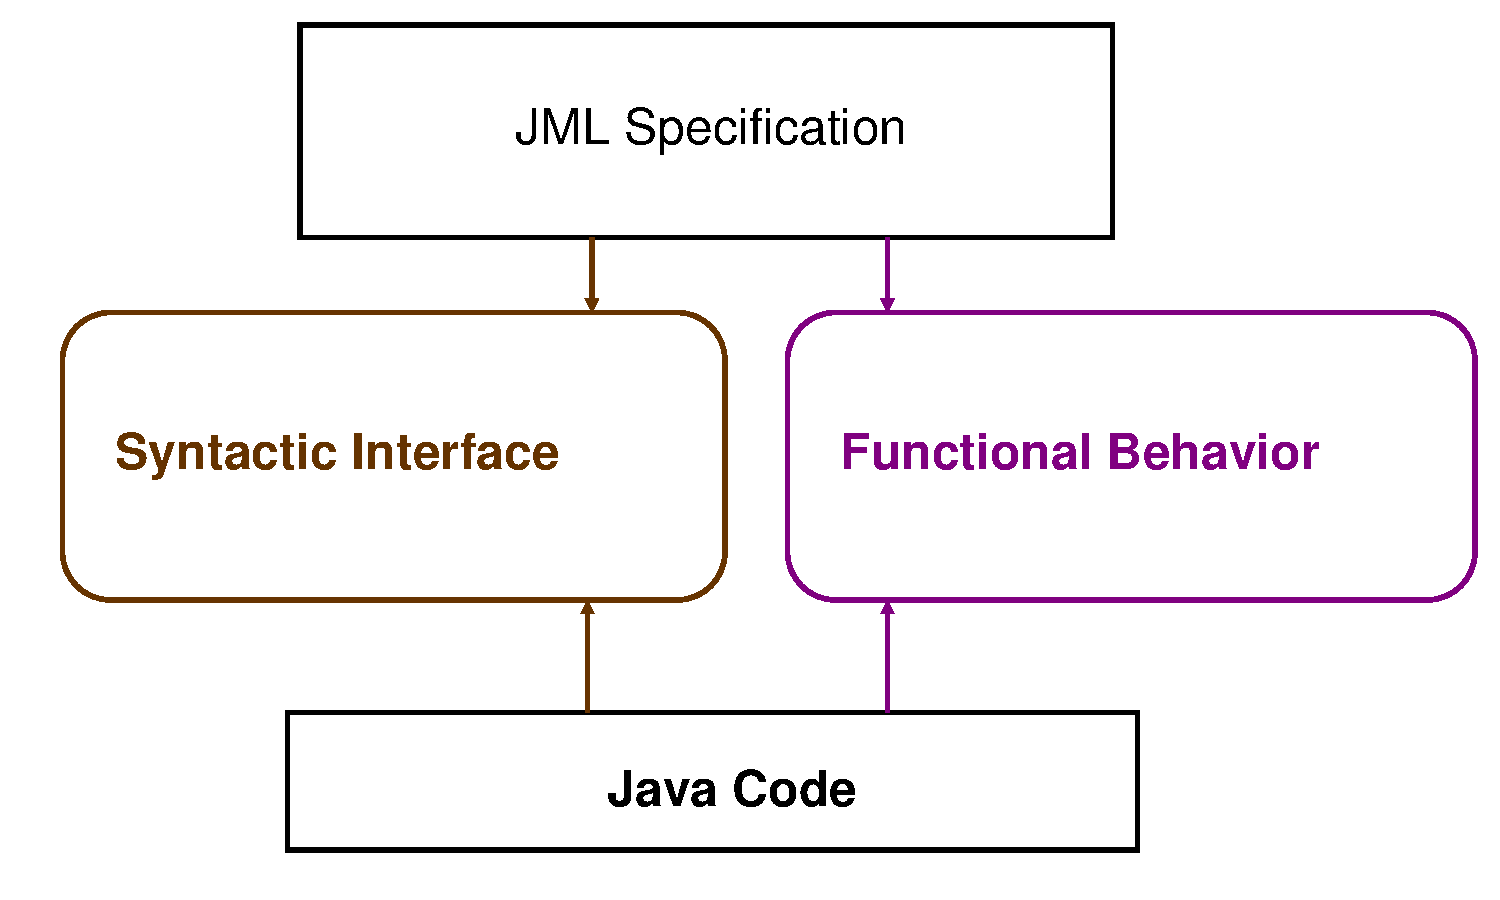
\includegraphics[width=4.25in]{if0}
\end{frame}

\begin{frame}
\frametitle{Interface Specification}
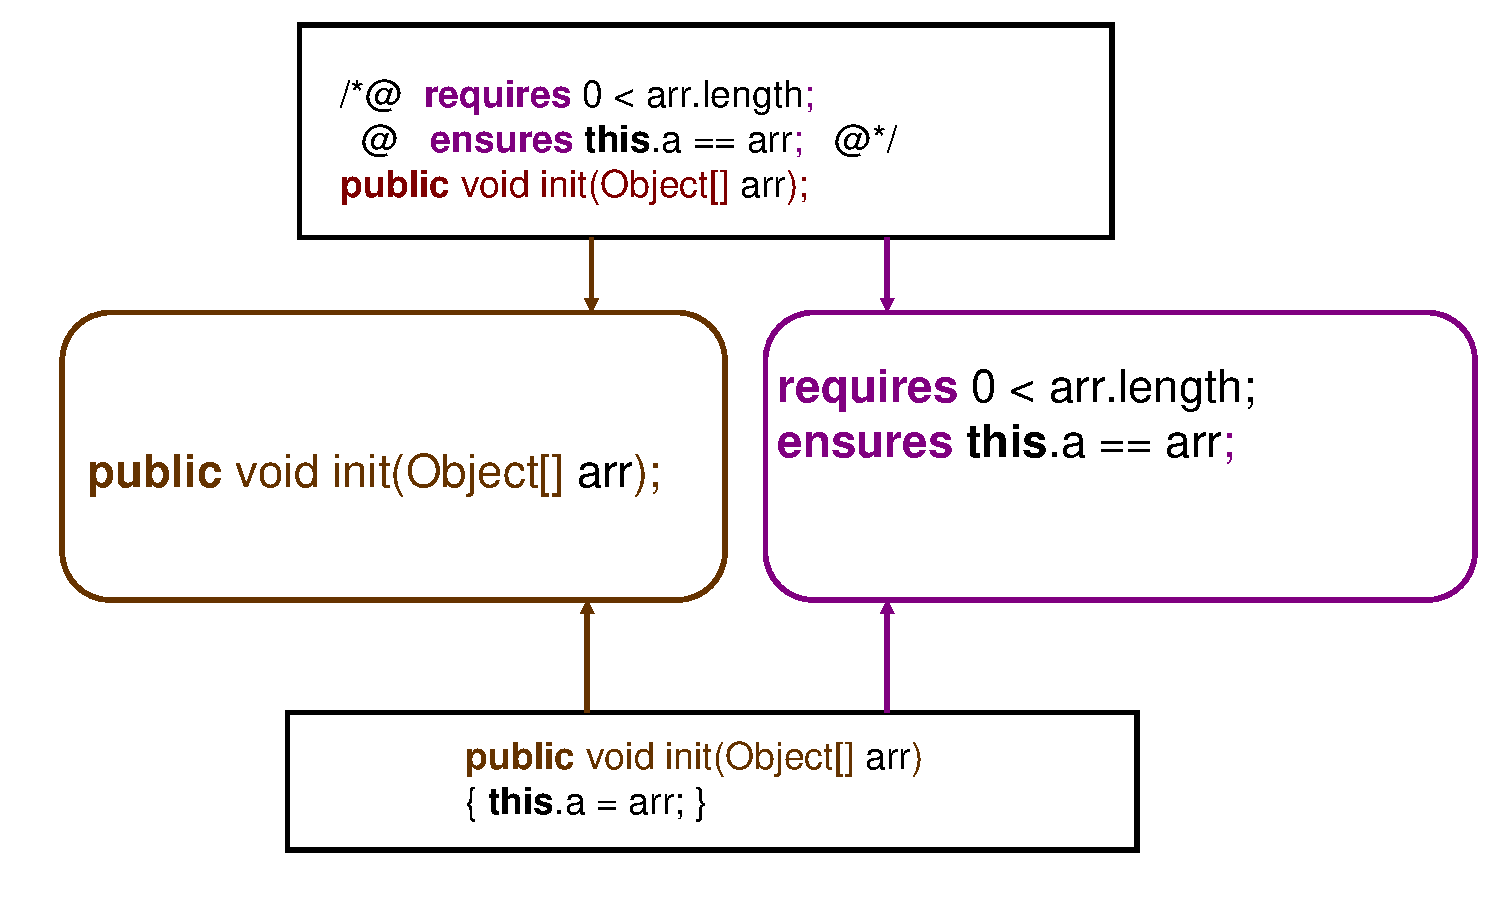
\includegraphics[width=4.25in]{if1}
\end{frame}

\begin{frame}
\frametitle{Like $\ldots$ But for Java and $\ldots$}
\begin{itemize}
\item
\textcolor{blue}{VDM}, but
\begin{itemize}
\item
OO features
\end{itemize}

\item
\textcolor{blue}{Eiffel}, but
\begin{itemize}
\item
Features for formal verification
\end{itemize}

\item
\textcolor{blue}{Spec\#}, but
\begin{itemize}
\item
Different invariant methodology
\item
More features for formal verification
\end{itemize}
\end{itemize}
\end{frame}

\begin{frame}
\frametitle{Unlike OCL and Z}

\begin{itemize}
\item
More Java-like syntax.

\item
Tailored to Java semantics.
\end{itemize}
\note{The JML features/differences make it easier for Java programmers
  to use JML and to read it.}
\end{frame}

\begin{frame}
\frametitle{Many Tools, One Language}
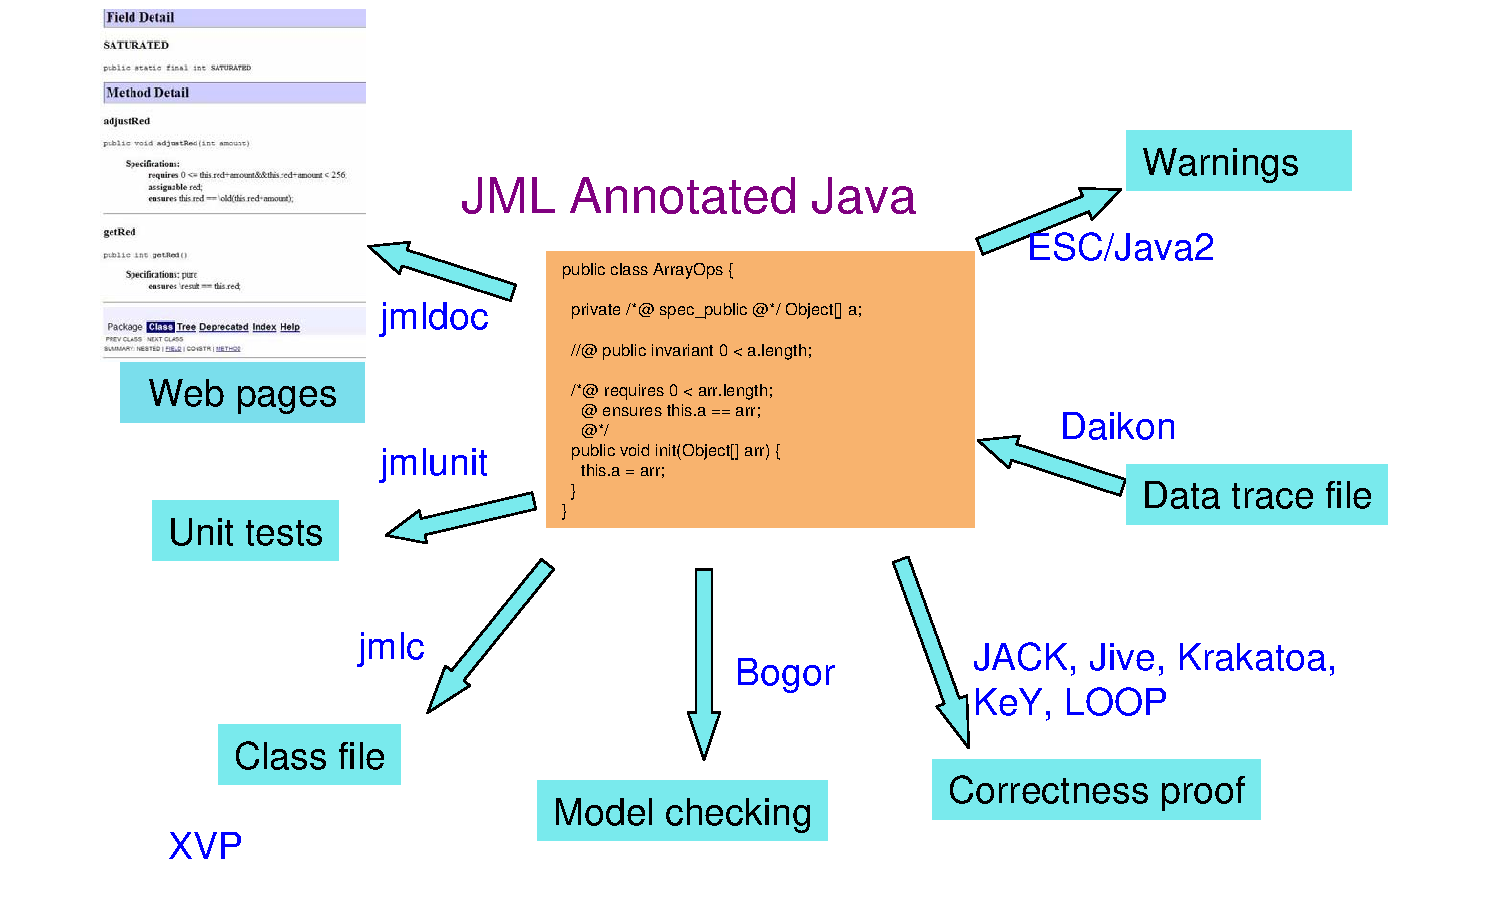
\includegraphics[width=4.25in]{tools-overview}
\end{frame}

\begin{frame}
\frametitle{How Tools Complement Each Other}
\begin{itemize}
\item
Different strengths:
\begin{itemize}
\item
Runtime checking --- real errors.

\item
Static checking --- better coverage.

\item
Verification --- guarantees.
\end{itemize}

\item
Usual ordering:
\begin{enumerate}
\item
One or both of:
\begin{itemize}
\item
Runtime checker (jmlc).

\item
Extended Static Checking (ESC/Java2).
\end{itemize}

\item
Verification tool (e.g., KeY, JACK, Jive).
\end{enumerate}
\end{itemize}
\note{You might want to use the RAC after ESC/Java2, or concurrently
  with it.
}
\end{frame}

\subsection[Interest]{Interest in JML}

\begin{frame}
\frametitle{Interest in JML}

\begin{itemize}
\item
Many tools.

\item
State of the art language.

\item
Large and open research community:
\begin{itemize}
\item
23 groups, worldwide.

\item
Over 135 papers.
\end{itemize}
\end{itemize}

See \href{http://www.jmlspecs.org}{jmlspecs.org}
\end{frame}

\begin{frame}[label=advantages]
\frametitle{Advantages of Working with JML}

\begin{itemize}
\item
Reuse language design.

\item
Ease communication with researchers.

\item
Share customers.
\end{itemize}

Join us!
\end{frame}

\begin{frame}[label=opportunities]
\frametitle{Opportunities in Working with JML}
\framesubtitle{Or: What Needs Work}

\begin{itemize}
\item
Tool development, maintenance.

\item
Extensible tool architecture.

\item
Unification of tools.
\end{itemize}
\end{frame}

\subsection[Finding More]{Where to Find More}

\begin{frame}
\frametitle{Where to Find More: \href{http://www.jmlspecs.org}{jmlspecs.org}}

Documents:
\begin{itemize}
\item
\href{ftp://ftp.cs.iastate.edu/pub/leavens/JML/jmldbc.pdf}{``Design by Contract with JML''}

\item
\href{http://dx.doi.org/10.1007/s10009-004-0167-4}{``An overview of JML tools and applications''}

\item
\href{http://doi.acm.org/10.1145/1127878.1127884}{``Preliminary Design of JML''}

\item
\href{http://dx.doi.org/10.1007/11901433}{``JML's Rich, Inherited Specifications for Behavioral Subtypes''}

\item
\href{http://www.jmlspecs.org/jmlrefman/jmlrefman_toc.html}{``JML Reference Manual''}
\end{itemize}

Also:
\begin{itemize}
\item
Examples, teaching material.

\item
Downloads, sourceforge project.

\item
Links to papers, etc.
\end{itemize}

\end{frame}

\section[R/W]{Reading and Writing JML Specifications}

\subsection[Lightweight]{Lightweight Specification of Functional Behavior}

\begin{frame}[fragile]
\frametitle{JML Annotations Comments $\neq$ Java Annotations}

JML annotation comments:
\begin{itemize}
\item
Line starting with \lstinline!//@!

\item
Between \lstinline!/*@! and \lstinline!@*/!,
ignoring \lstinline!@!'s starting lines.
\end{itemize}

First character must be \lstinline!@!

\note{Java annotations are not in comments.

We are experimenting with putting JML in Java annotations, but that's
not standard and doesn't work with any tools at present.}
\end{frame}

\begin{frame}
\frametitle{Most Important JML Keywords}

Top-level in classes and interfaces:
\begin{itemize}
\item
\lstinline!invariant!

\item
\lstinline!spec_public!

\item
\lstinline!nullable!
\end{itemize}

For methods and constructors:
\begin{itemize}
\item
\lstinline!requires!

\item
\lstinline!ensures!

\item
\lstinline!assignable!

\item
\lstinline!pure!
\end{itemize}
\end{frame}

\begin{frame}
\frametitle{Example: BoundedStack}

\begin{example}
Specify bounded stacks of objects.
\end{example}

\note{See the file BoundedStack.java}
\end{frame}

\begin{frame}[fragile]
\frametitle{BoundedStack's Data and Invariant}
\lstinputlisting[linerange={1-13}]{examples/BoundedStack.java}
\note{Explain notation. Stress client view.

The elems field is nullable, to allow the elements to be null.
Without this the JML default is that they are both non-null.

The part of the invariant that talks about the elements at indexes
at size and larger being null could reasonably be private, but we
haven't introduced that concept yet.
}
\end{frame}

\begin{frame}[fragile]
\frametitle{BoundedStack's Constructor}
\lstinputlisting[linerange={14-20}]{examples/BoundedStack.java}
\end{frame}

\begin{frame}[fragile]
\frametitle{BoundedStack's push Method}
\lstinputlisting[linerange={22-33}]{examples/BoundedStack.java}
\note{Talk about the assignable clause and the postcondition
and how they relate to the code.

Subexpressions of assignable clause store-ref expressions are
evaluated in the pre-state.

The \lstinline!ensures_redundantly! is there becuase that
postcondition follows from the assignable clause.
}
\end{frame}

\begin{frame}[fragile]
\frametitle{BoundedStack's pop Method}
\lstinputlisting[linerange={35-46}]{examples/BoundedStack.java}
\end{frame}

\begin{frame}[fragile]
\frametitle{BoundedStack's top Method}
\lstinputlisting[linerange={48-55}]{examples/BoundedStack.java}
\end{frame}

\begin{frame}[fragile]
\frametitle{spec\_public, nullable, and invariant}

\lstinline!spec_public!
\begin{itemize}
\item
Public visibility.

\item
Only public for specification purposes.
\end{itemize}

\note{\lstinline!spec_public! actually a syntactic sugar.}

\lstinline!nullable!
\begin{itemize}
\item
field (and array elements) may be null.

\item
Default is \lstinline!non_null!.
\end{itemize}

\lstinline!invariant! must be:
\begin{itemize}
\item
True at end of constructor.

\item
Preserved by each method.
\end{itemize}

\note{\par
Helper methods are an exception to invariant preservation, which
  we'll discuss later, so no need to talk about it now.}
\end{frame}

\begin{frame}[fragile]
\frametitle{requires and ensures}

\lstinline!requires! clause:
\begin{itemize}
\item
Precondition.

\item
Obligation on callers, after parameter passing.

\item
Assumed by implementor.
\end{itemize}

\lstinline!ensures! clause:
\begin{itemize}
\item
Postcondition.

\item
Obligation on implementor, at return.

\item
Assumed by caller.
\end{itemize}
\end{frame}

\begin{frame}
\frametitle{Semantics of Requires and Ensures}
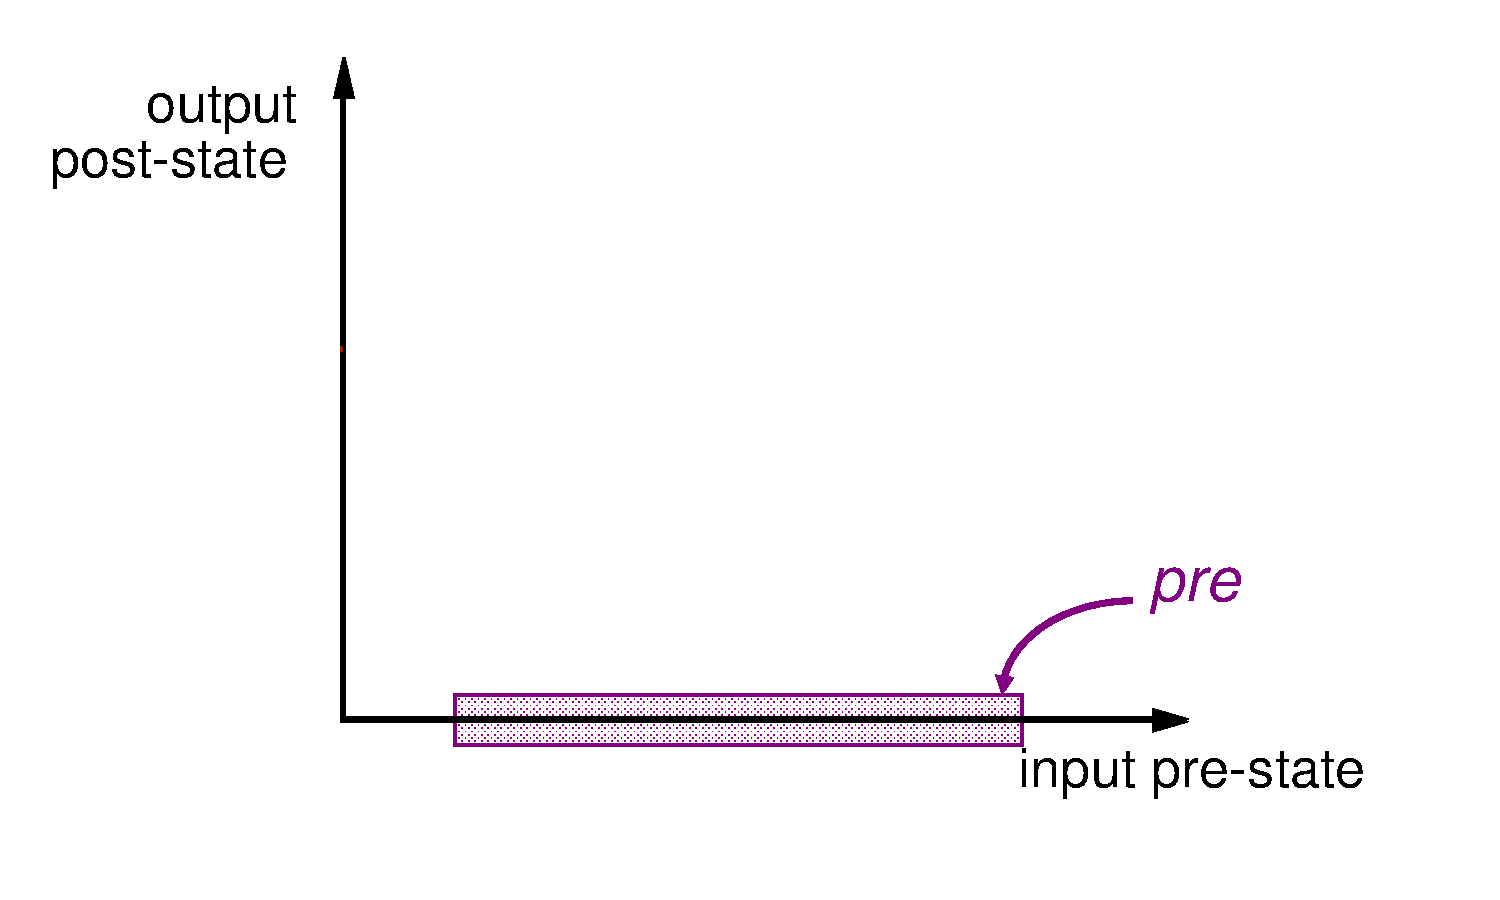
\includegraphics[width=4.25in]{requires}
\end{frame}

\begin{frame}
\frametitle{Semantics of Requires and Ensures}
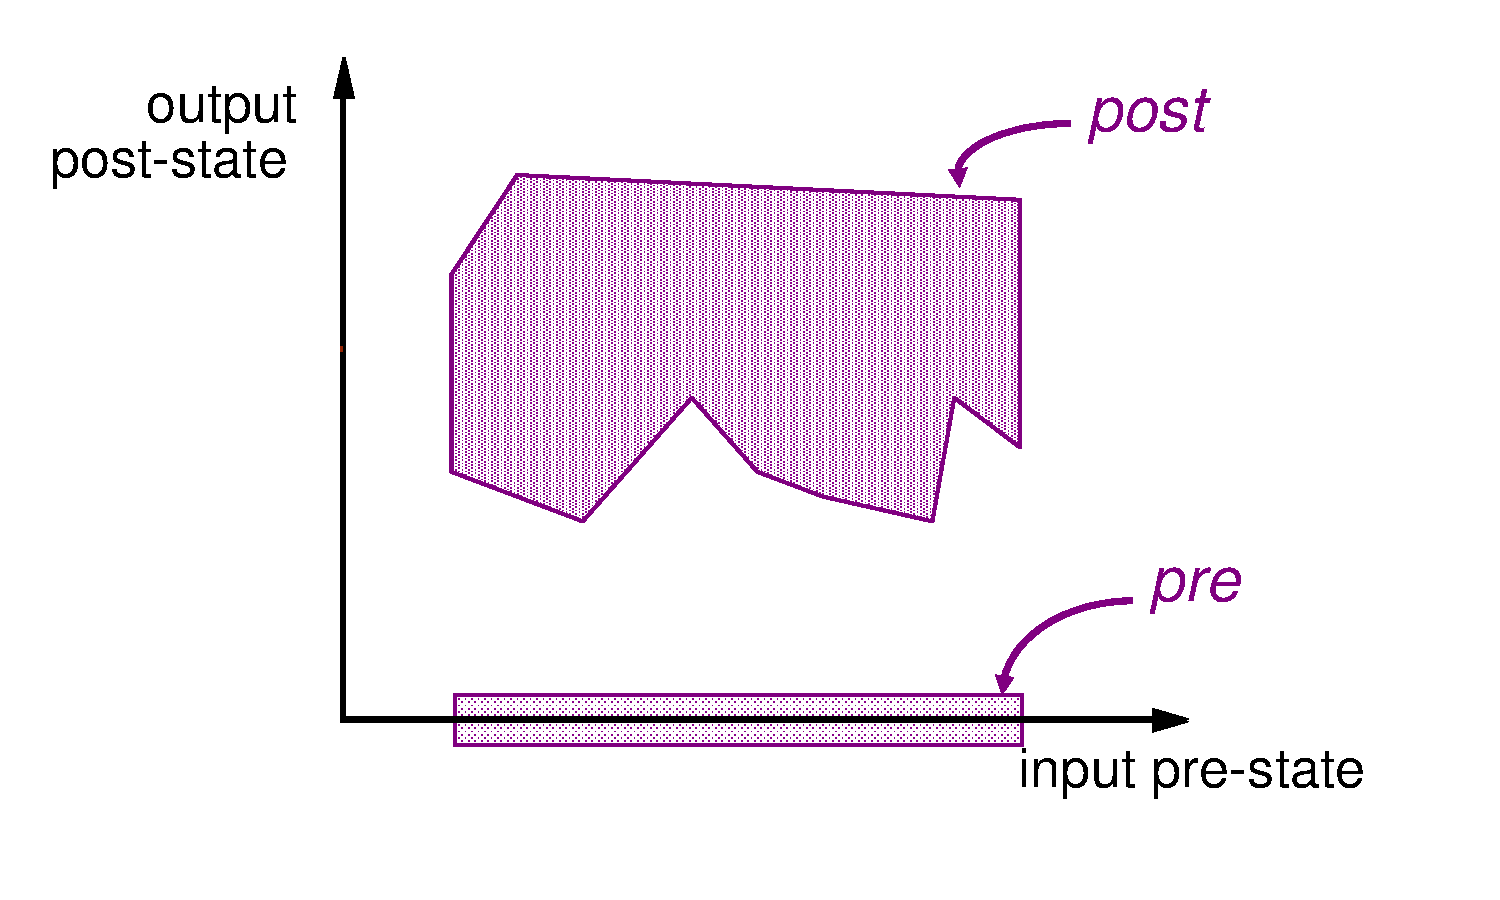
\includegraphics[width=4.25in]{ensures}
\end{frame}

\begin{frame}
\frametitle{Semantics of Requires and Ensures}
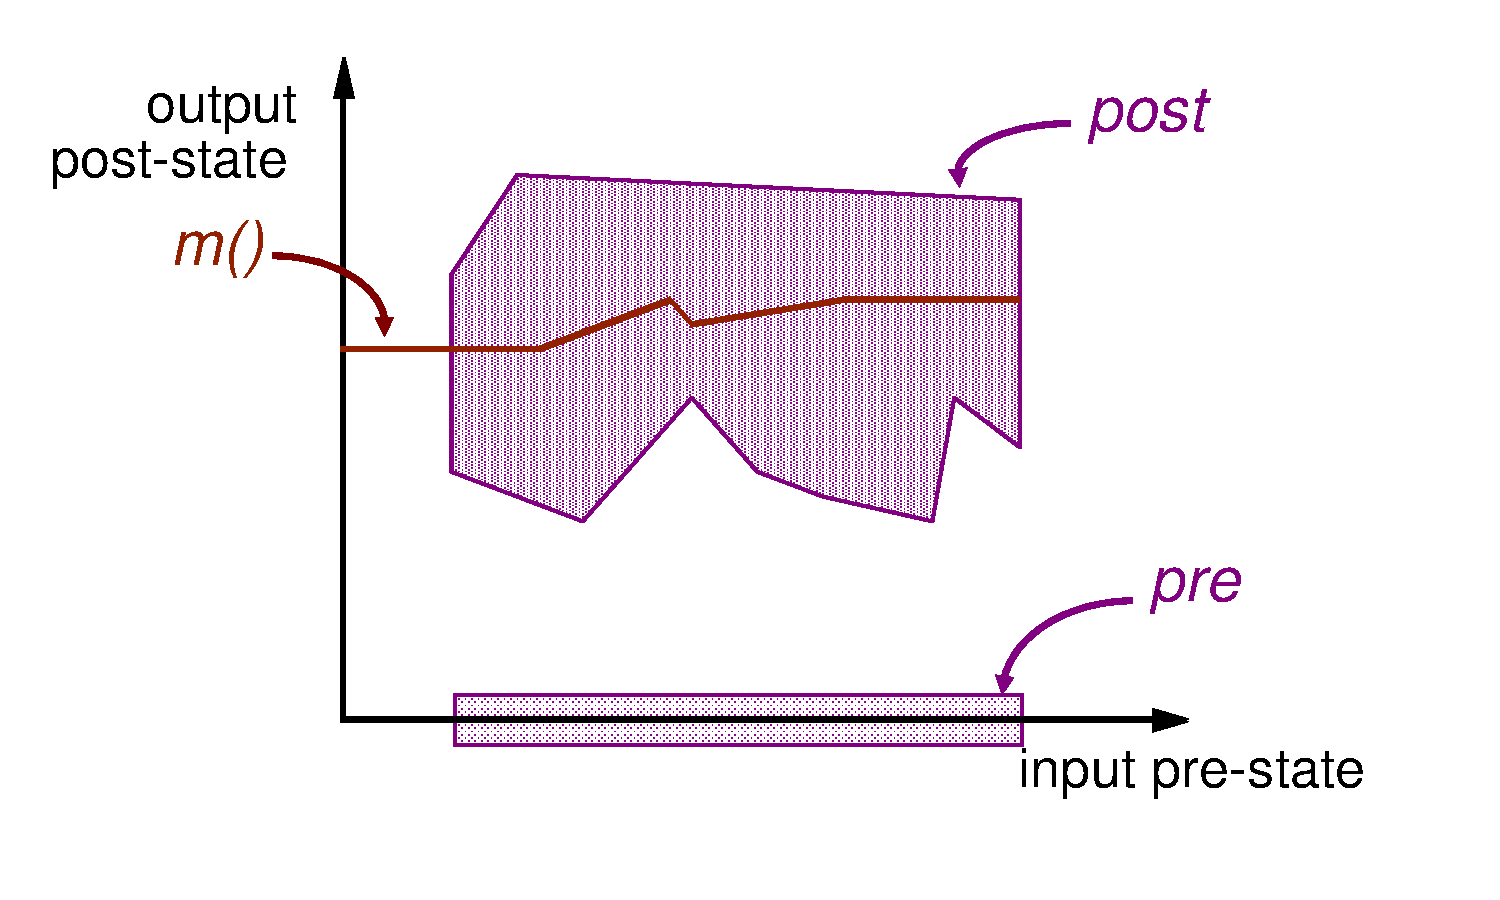
\includegraphics[width=4.25in]{correctimpl}
\end{frame}

\begin{frame}[fragile]
\frametitle{assignable and pure}

\lstinline!assignable!
\begin{itemize}
\item
Frame axiom.

\item
Locations (fields) in pre-state.

\item
New object fields not covered.

\item
Mostly checked statically.

\item
Synonyms: \lstinline!modifies!, \lstinline!modifiable!
\end{itemize}

\lstinline!pure!
\begin{itemize}
\item
No side effects.

\item
Implies \lstinline!assignable \nothing!

\item
Allows method's use in specifications.
\end{itemize}
\note{Note that pure is a modifier for methods, not a clause.}
\end{frame}

\begin{frame}[fragile]
\frametitle{Assignable is a Shorthand}
\begin{lstlisting}[mathescape=true]
  assignable gender;
  ensures gender.equals(g);
\end{lstlisting}

means

\begin{lstlisting}[mathescape=true]
  ensures \only_assigned(gender)
       && gender.equals(g);
\end{lstlisting}
\end{frame}

\begin{frame}[fragile,label=redundantly]
\frametitle{Redundant Clauses}

E.g., \lstinline!ensures_redundantly!
\begin{itemize}
\item
Alerts reader.

\item
States something to prove.

\item
Must be implied by:
\begin{itemize}
\item
\lstinline!ensures! clauses,

\item
\lstinline!assignable! clause,

\item
\lstinline!invariant!, and

\item
JML semantics.
\end{itemize}
\end{itemize}

Also \lstinline!requires_redundantly!, etc.

\note{There is a flag on jmlc to avoid checking redundant
specifications, but they are checked by default.
}
\end{frame}

\begin{frame}[fragile]
\frametitle{Multiple Clauses}

Semantics:

\begin{lstlisting}[mathescape=true]
  requires $P$;
  requires $Q$;
\end{lstlisting}

is equivalent to:

\begin{lstlisting}[mathescape=true]
  requires $P$ && $Q$;
\end{lstlisting}

Similarly for \lstinline!ensures!, \lstinline!invariant!.

~

Note: runtime checker gives better errors with multiple clauses.

\note{For assignable, semantics is the union.}
\end{frame}

\begin{frame}[fragile]
\frametitle{Defaults for Omitted Clauses}

\begin{itemize}
\item
\lstinline!invariant true;!

\item
\lstinline!requires true;!

\item
\lstinline!assignable \everything;!

\item
\lstinline!ensures true;!
\end{itemize}
\note{Strictly speaking, the defaults listed here are a lie.
  For lightweight specifications the defaults are all
  ``not specified.''  The listed defaults are
  actually the defaults for heavyweight specifications
  (that use the \lstinline!behavior! or \lstinline!normal_behavior! keywords).
  However, the tools treat them this way.
}
\end{frame}

\begin{frame}[fragile]
\frametitle{Expression Keywords}

\begin{itemize}
\item
\lstinline!\result! ~~ = ~~ method's return value.

\item
\lstinline[mathescape=true]!\old($E$)! ~~ = ~~ pre-state value of $E$.

\item
\lstinline[mathescape=true]!(\forall T x; $P$; $Q$)!
~~ = ~~ $\bigwedge \{ Q \mid x \in T \wedge P \}$

\item
\lstinline[mathescape=true]!(\exists T x; $P$; $Q$)!
~~ = ~~ $\bigvee \{ Q \mid x \in T \wedge P \}$

\item
\lstinline[mathescape=true]!(\min T x; $P$; $E$)!
~~ = ~~ $\min \{E \mid x \in T \wedge P \}$

\item
\lstinline[mathescape=true]!(\sum T x; $P$; $E$)!
~~ = ~~ $\sum \{E \mid x \in T \wedge P \}$

\item
\lstinline[mathescape=true]!(\num_of T x; $P$; $Q$)!
~~ = ~~ $\sum \{1 \mid x \in T \wedge P \wedge Q\}$

\item
$\ldots$
\end{itemize}
\note{We use the backslashes to avoid reserving words in expression contexts.

This is more than we need now, but stress the regular pattern of
the quantifiers, with a domain and range predicate.

The listeners of this tutorial will be able to use \texttt{\textbackslash}\lstinline!num_of! later.

The \texttt{\textbackslash}\lstinline!num_of! quantifier actually produces a long, not int, result.
}
\end{frame}

\subsection[Exercise]{Specifying a Type}

\begin{frame}[fragile]
\frametitle{Steps for Specifying a Type for Public Clients}

\begin{enumerate}
\item
Specify data (\lstinline!spec_public! fields).

\item
Specify a \lstinline!public invariant!.

\item
Specify each public method using:

\begin{enumerate}
\item
\lstinline!requires!.

\item
\lstinline!assignable! (or \lstinline!pure!).

\item
\lstinline!ensures!.
\end{enumerate}
\end{enumerate}
\note{The invariant can be omitted if not needed, as can the requires clause.}
\end{frame}

\begin{frame}[fragile]
\frametitle{Exercise: Specify BagOfInt (7 minutes)}

\begin{exercise}
Specify the following:

\rm
\lstinputlisting[language=Java,commentstyle=\itshape]{examples/BagOfInt.jml-refined}
\end{exercise}
\note{We have somewhat artificially decided on data structures here,
  since we haven't introduced JML's model features.

The intent is that \texttt{a} holds the elements that are not yet deleted,
and \texttt{n} tells the number of elements that haven't yet been
deleted.
}
\end{frame}

\begin{frame}<beamer>[fragile]
\frametitle{My Solution: BagOfInt's Data}

\lstinputlisting[linerange={2-2,4-9}]{examples/BagOfInt.jml}
\note{Note that we're using the default \lstinline!non_null! for
\lstinline!a! instead of making it \lstinline!nullable!.
This is because there are no elements of reference types.
}
\end{frame}

\begin{frame}<beamer>[fragile]
\frametitle{My Solution: BagOfInt's Constructor}

\lstinputlisting[linerange={11-11,13-17}]{examples/BagOfInt.jml}
\note{It would be a bad specification to make \texttt{a} and
  \texttt{input} be aliases.
}
\end{frame}

\begin{frame}<beamer>[fragile]
\frametitle{My Solution: Method occurrences}

\lstinputlisting[linerange={19-19,21-24}]{examples/BagOfInt.jml}
\end{frame}

\begin{frame}<beamer>[fragile]
\frametitle{My Solution: Method extractMin}

\lstinputlisting[linerange={26-26,28-40}]{examples/BagOfInt.jml}
\note{The frame is written to allow one to either replace/copy
 the entire array or to assign to some elements.

Note that one could use \texttt{\textbackslash}\lstinline!num_of!
directly instead of calling \texttt{occurrences} in the specification,
however, this illustrates how to do that, and makes the specification
much shorter.
}
\end{frame}


\subsection[Tools]{Basic Tool Use}  % demo + exercise

\begin{frame}
\frametitle{Goals of the Tools}
\begin{description}[ESC/Java2:]
\item[jmlc:]
Find violations at runtime.

\item[jmlunit:]
Aid/automate unit testing.

\item[ESC/Java2:]
Warn about likely runtime exceptions and violations.
\end{description}
\end{frame}

\begin{frame}
\frametitle{Getting the Tools}

Links to all tools:
\begin{itemize}
\item
\href{http://www.jmlspecs.org/}{jmlspecs.org}'s download page.
\end{itemize}


Individual tools:
\begin{itemize}
\item
Common JML tools \\
\href{http://sourceforge.net/projects/jmlspecs/}{sourceforge.net/projects/jmlspecs/}

\item
ESC/Java2 Eclipse plugin update site \\
\href{http://sort.ucd.ie/www/escjava-eclipse/updates}{http://sort.ucd.ie/www/escjava-eclipse/updates}
\end{itemize}
\end{frame}

\begin{frame}[fragile]
\frametitle{Using jmlc, the Runtime Checker}

\begin{example}
\begin{verbatim}
$ jmlc -Q -e BagOfInt.java BagOfIntMain.java
$ jmlrac BagOfIntMain
\end{verbatim}
\end{example}
\note{This should be a demo, with Emacs or Eclipse.

We're using CLASSPATH=. because of the use of the unnamed package;
for other packages, we have to be careful, as with Java.

(You might want to show what happens with compiling with javac and
running with java (the VM) first, to see what difference using jmlc makes.)

The -Q flag shuts jmlc up somewhat.  The -e flag turns on universes.

These flags are valid for JML Common Tools release 5.4.

There are manual pages for each of the tools.
}
\end{frame}

\begin{frame}[fragile]
\frametitle{Writing Tests Using Assert}

\lstinputlisting[linerange={4-17}]{examples/BagOfIntMain.java}
\note{It's much better to use assert than to try to look at output!

You can use Java's assert too, but there are advantages to using
JML's assert, as is done here.
}
\end{frame}

\begin{frame}[fragile]
\frametitle{Using jmlc, the Runtime Checker}

{\small
\begin{verbatim}
org...JMLInternalExceptionalPostconditionError:
 by method BagOfInt.occurrences regarding spec...s at
   File "BagOfInt.jml", line 21, character 14, when
    'jml$e' is ...ArrayIndexOutOfBoundsException: 6
   at BagOfInt.main(BagOfInt.java:2120)
Exception in thread "main" 
\end{verbatim}
% $
}
\lstinputlisting[linerange={21-24},numbers=left,numberstyle=\small]{examples/BagOfInt.jml}
\end{frame}

\begin{frame}[fragile]
\frametitle{Using jmlc with jmlunit}

\begin{example}
CLASSPATH includes:
\begin{itemize}
\item
\texttt{.}

\item
\texttt{junit.jar} (version 3.8.1)

\item
\texttt{JML/bin/jml-release.jar}
\end{itemize}

\begin{verbatim}
$ jmlunit -i BagOfInt.java
\end{verbatim}
% $

Edit \lstinline!BagOfInt_JML_TestData.java!

\begin{verbatim}
$ javac BagOfInt_JML_Test*.java
$ jmlc -Q -e BagOfInt.java
$ jmlrac BagOfInt_JML_Test
\end{verbatim}
% $
\end{example}
\note{This should be a demo.

Note you have to compile with jmlc \emph{after} compiling with javac,
since javac will compile the executable without RAC.  

Put in data for
ints: 3, 4, 5, 10, \\

arrays: new int[] \{3, 4, 2, 3, 3\}, \{0, 10, 20, 30, 10\}, \{\}, and \\

bags with those arrays as initial values:
\lstinline!case N: return new BagOfInt(...);!.
}
\end{frame}

\begin{frame}[fragile]
\frametitle{Using jmlc with jmlunit}

{\small
\begin{verbatim}
.....F.F.F.F.F.F.F.F.F.F.F.F.F.F........F.F.....
Time: 0.01
There were 16 failures:
1) occurrences:0(BagOfInt_JML_Test$TestOccurrences)
  junit.framework.AssertionFailedError:
    Method 'occurrences' applied to
    Receiver: {3, 4, 2, 3, 3}
    Argument i: 0
Caused by: ...JMLExitExceptionalPostconditionError:
by: method BagOfInt.occurrences regarding spec...s at
   File "BagOfInt.jml", line 21, character 14, when
    'jml$e' is ...ArrayIndexOutOfBoundsException: 5
\end{verbatim}
% $
}
\end{frame}

\begin{frame}[fragile]
\frametitle{Using ESC/Java2}

\begin{example}
\begin{verbatim}
$ CLASSPATH=.
$ export CLASSPATH
$ escjava2 -nonNullByDefault BagOfInt.java
\end{verbatim}
% $
\end{example}
\note{This should be a demo, with Emacs or Eclipse.

To get the Eclipse demo to run on Windows, I had to tell Eclipse about the
Simplify executable location explicitly in the preferences.
See Window/Preferences/Java/EscJava2 in the Eclipse menus.
}
\end{frame}

\begin{frame}[fragile]
\frametitle{Using ESC/Java2}

{\small
\begin{verbatim}
BagOfInt ...
  Prover started:0.03 s 15673776 bytes
    [2.013 s 15188656 bytes]

BagOfInt: BagOfInt(int[]) ...
---------------------------------------------------
BagOfInt.java:11: Warning: 
      Postcondition possibly not established (Post)
  }
  ^
Associated declaration is 
".\BagOfInt.jml", line 14, col 6:
    @ ensures (\forall int i; 0 <= i && i < n;
      ^
\end{verbatim}
}
\end{frame}

\subsection[Tips/Pitfalls]{Tips and Pitfalls}

\begin{frame}
\frametitle{Tip: Use JML Assert Statements}

\begin{columns}[t]
\column{.5\textwidth}
\begin{block}{JML assert statements}
\begin{itemize}
\item
All JML features.

\item
No side effects.
\end{itemize}
\end{block}

\column{.5\textwidth}
\begin{block}{Java assert statements}
\begin{itemize}
\item
Only Java expressions.

\item
Can have side effects.
\end{itemize}
\end{block}
\end{columns}

\note{JML features include quantifiers, and model fields.}
\end{frame}

\begin{frame}[fragile]
\frametitle{Tip: Use JML Assume Statements}

\lstinline!assume! $P$\texttt{;}

\begin{itemize}
\item
Claims $P$ is true.

\item
Checked by the RAC like \lstinline!assert! $P$\texttt{;}

\item
Blame other party if false.

\item
Assumed by ESC/Java and static tools.
\end{itemize}
\note{There are differences in static checkers, such as ESC/Java, and
  in error messages and exceptions from the RAC, however.
}
\end{frame}

\begin{frame}[fragile]
\frametitle{Assume Statements and Verification}

\begin{lstlisting}[mathescape=true]
//@ requires $P$;
//@ ensures $Q$;
public void m() {
  $S$
}
\end{lstlisting}

~~generates:

\begin{lstlisting}[mathescape=true]
public void m() {
  //@ assume $P$;
  $S$
  //@ assert $Q$;
}
\end{lstlisting}
\end{frame}

\begin{frame}[fragile]
\frametitle{Assume Statements and Verification}

\begin{lstlisting}[mathescape=true]
//@ requires $P$;
//@ ensures $Q$;
public void m() {
  $S$
}
\end{lstlisting}

~~generates:

\begin{lstlisting}[mathescape=true]
//@ assert $P$;
o.m();
//@ assume $Q$;
\end{lstlisting}

\end{frame}

\begin{frame}
\frametitle{Pitfall: Aliasing in Java}
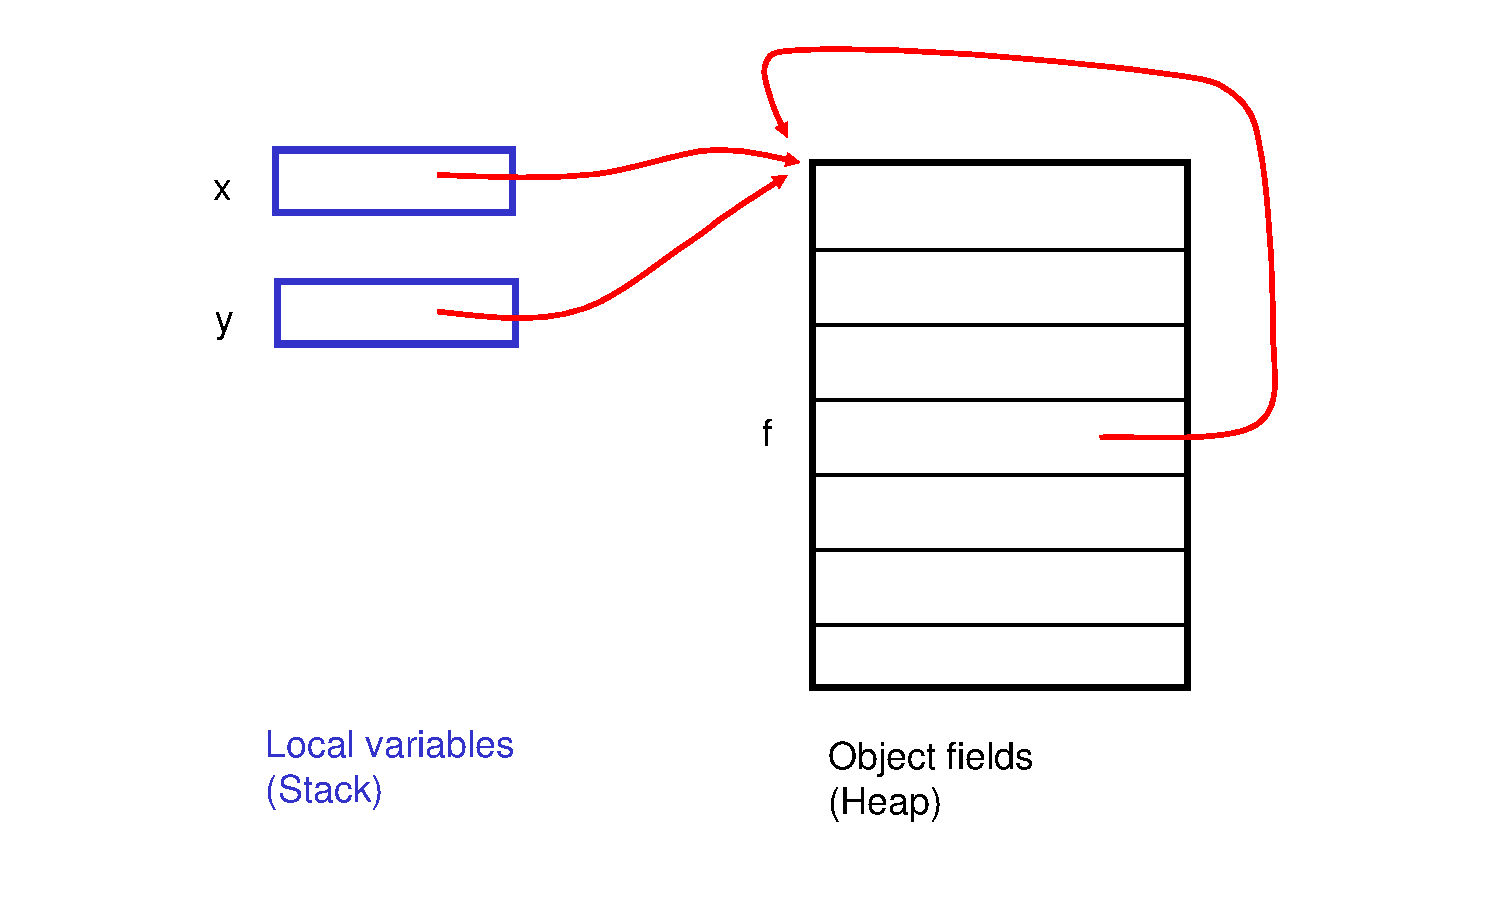
\includegraphics[width=4.25in]{aliasxy}
\end{frame}

\begin{frame}
\frametitle{Aliasing and Object Identity}
\framesubtitle{JML Uses Java's Indirect Model for Objects}

For objects $x$ and $y$, $x$ \texttt{==} $y$ means:
\begin{itemize}
\item
$x$ and $y$ have same address.

\item
$x$ and $y$ are aliased.

\item
Changing of $x.f$ also changes $y.f$.
\end{itemize}

Aliasing caused by:
\begin{itemize}
\item
Assignment ($x$ \texttt{=} $y$).

\item
Method calls 
\begin{itemize}
\item
Passing field $o.y$ to formal $x$.

\item
Passing both $x$ and $y$ to different formals.

\item
Etc.
\end{itemize}
\end{itemize}
\end{frame}

\begin{frame}[fragile]
\frametitle{Pitfall: Aliasing}

\begin{question}
What's wrong with this? \uncover<2->{How to fix it?}

\rm
\lstinputlisting{examples/Counter.java}
\end{question}
\note<1>{The postcondition may fail.  ESC/Java shows this.

Note: in Java variables of different types can be aliased, 
due to multiple inheritance of interface types.
}
\end{frame}

\begin{frame}<beamer>[fragile]
\frametitle{Revised Counter to Fix the Problem}

\lstinputlisting{examples/Counter2.java}
\end{frame}

\begin{frame}[fragile]
\frametitle{Pitfall: Representation Exposure}

\lstinputlisting[linerange={1-14}]{examples/SortedInts.java}
\end{frame}

\begin{frame}[fragile]
\frametitle{Pitfall: Representation Exposure}

\begin{question}
What's wrong with this? \uncover<2->{How to fix it?}

\rm
\lstinputlisting[linerange={4-6}]{examples/SortedInts.java}
\lstinputlisting[linerange={16-22}]{examples/SortedInts.java}
\end{question}
\note<1>{The invariant may not hold on entry to the method, 
due to representation exposure.
}
\end{frame}

\begin{frame}<beamer>[fragile]
\frametitle{Revised SortedInts Using Universes (jmlc)}

\lstinputlisting[linerange={1-3}]{examples/SortedInts2.java}
\note{This solution is based on the Universe type/ownership system 
from Peter M\"{u}ller's group (Werner Dietl) at ETH.}
\end{frame}

\begin{frame}<beamer>[fragile]
\frametitle{Revised Using Universes (jmlc)}

\lstinputlisting[linerange={16-29}]{examples/SortedInts2.java}
\end{frame}

\begin{frame}<beamer>[fragile]
\frametitle{Revised Using Owner (ESC/Java2)}

\lstinputlisting[linerange={1-4}]{examples/SortedInts3.java}
\end{frame}

\begin{frame}<beamer>[fragile]
\frametitle{Revised Using Owner (ESC/Java2)}

\lstinputlisting[linerange={17-27}]{examples/SortedInts3.java}
\end{frame}

\begin{frame}<beamer>[fragile]
\frametitle{Revised Using Owner (ESC/Java2)}

\lstinputlisting[linerange={27-33}]{examples/SortedInts3.java}
\note{Owner is a ghost field, so assigned to by a \lstinline!set! statement.}
\end{frame}

\begin{frame}
\frametitle{Pitfall: Undefined Expressions}
\begin{question}
What's wrong with this? How to fix it?

\rm
\lstinputlisting[linerange={1-10}]{examples/ScreenPoint.java}
\end{question}
\note{The array out of bounds error is something that ESC/Java2
  detects, but only in the code.  Try it.
}
\end{frame}

\begin{frame}
\frametitle{Protective Version of ScreenPoint}
\lstinputlisting[linerange={1-11}]{examples/ScreenPoint2.java}
\note{See papers by Leavens and Wing on protective interface
  specifications, and papers by Chalin on the semantics of undefined
  expressions. 
}
\end{frame}

\begin{frame}[fragile]
\frametitle{Writing Protective Specifications}

\begin{itemize}
\item
Clauses evaluated left to right.

\item
Short-circuit operators can prevent evaluation.
\begin{itemize}
\item
$G$ \lstinline!&&! $P$, $G$ \lstinline!||! $P$

\item
$G$ \lstinline!==>! $P$, $G$ \lstinline!<==! $P$
\end{itemize}

\item
Use multiple clauses (equivalent to \lstinline!&&!).
\end{itemize}
\note{\lstinline!==>! is implication, and 
      \lstinline!<==! is reverse implication. 
}
\end{frame}


\subsection[Spec Cases]{Multiple Specification Cases}

\begin{frame}
\frametitle{Multiple Specification Cases}

\begin{itemize}
\item
For different preconditions.

\item
May overlap.

\item
Used to specify exceptions.

\item
Used with specification inheritance.
\end{itemize}
\note{This idea first appears in Jeannette Wing's 1983 Ph.D. dissertation.}
\end{frame}

\begin{frame}
\frametitle{Multiple Specification Cases}
\lstinputlisting[linerange={3-14}]{examples/Aging.java}
\end{frame}

\begin{frame}
\frametitle{Semantics of Multiple Cases}
\transdissolve[duration=0.5]
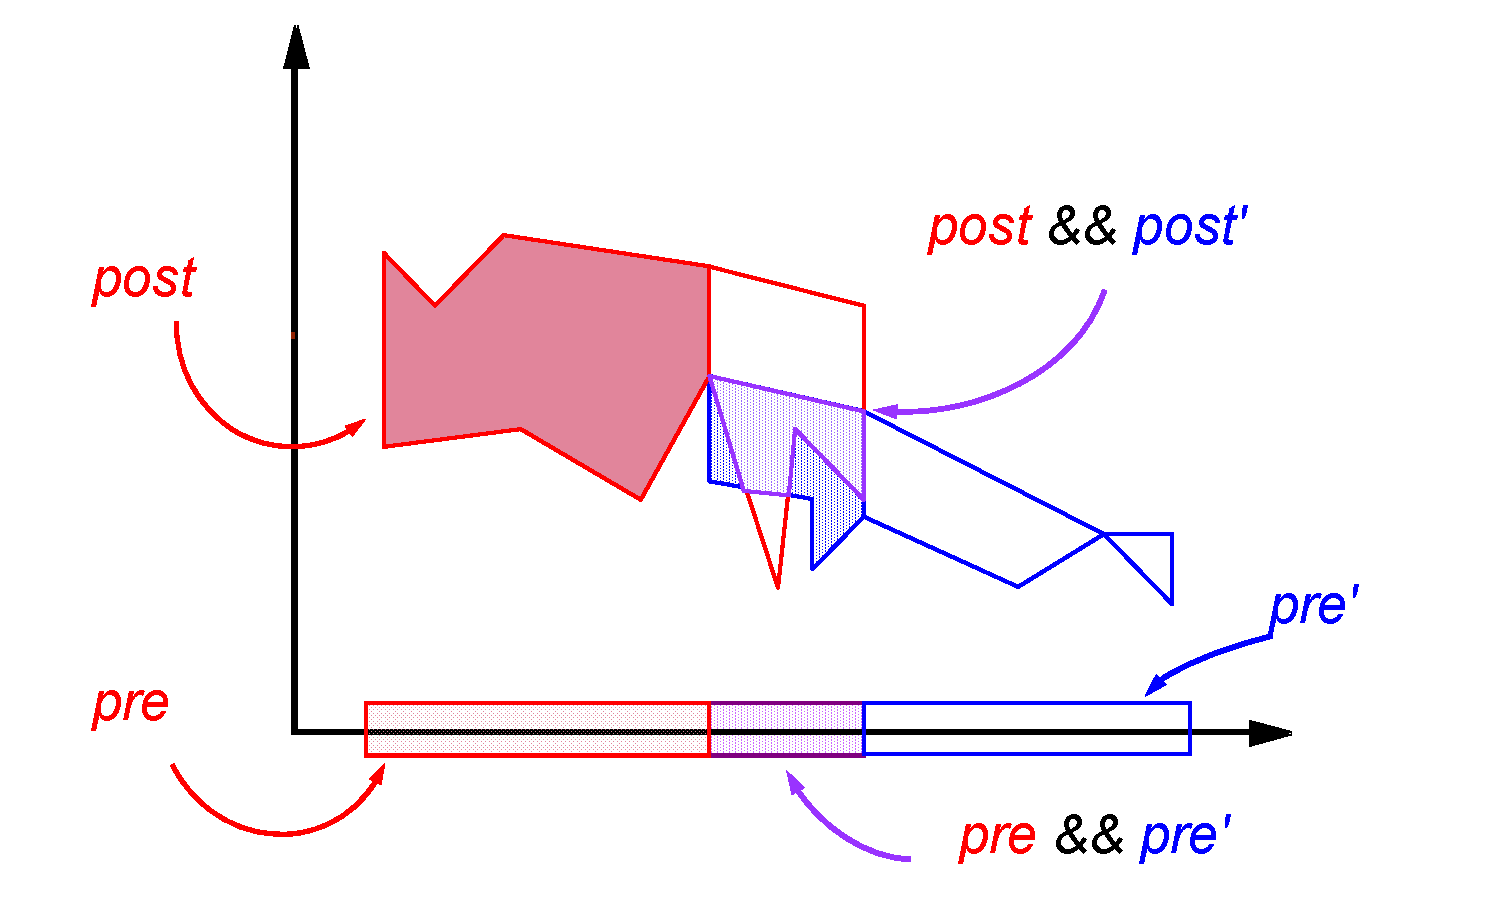
\includegraphics[width=4.25in]{join-both}
\end{frame}

\begin{frame}
\frametitle{Semantics of Multiple Cases}
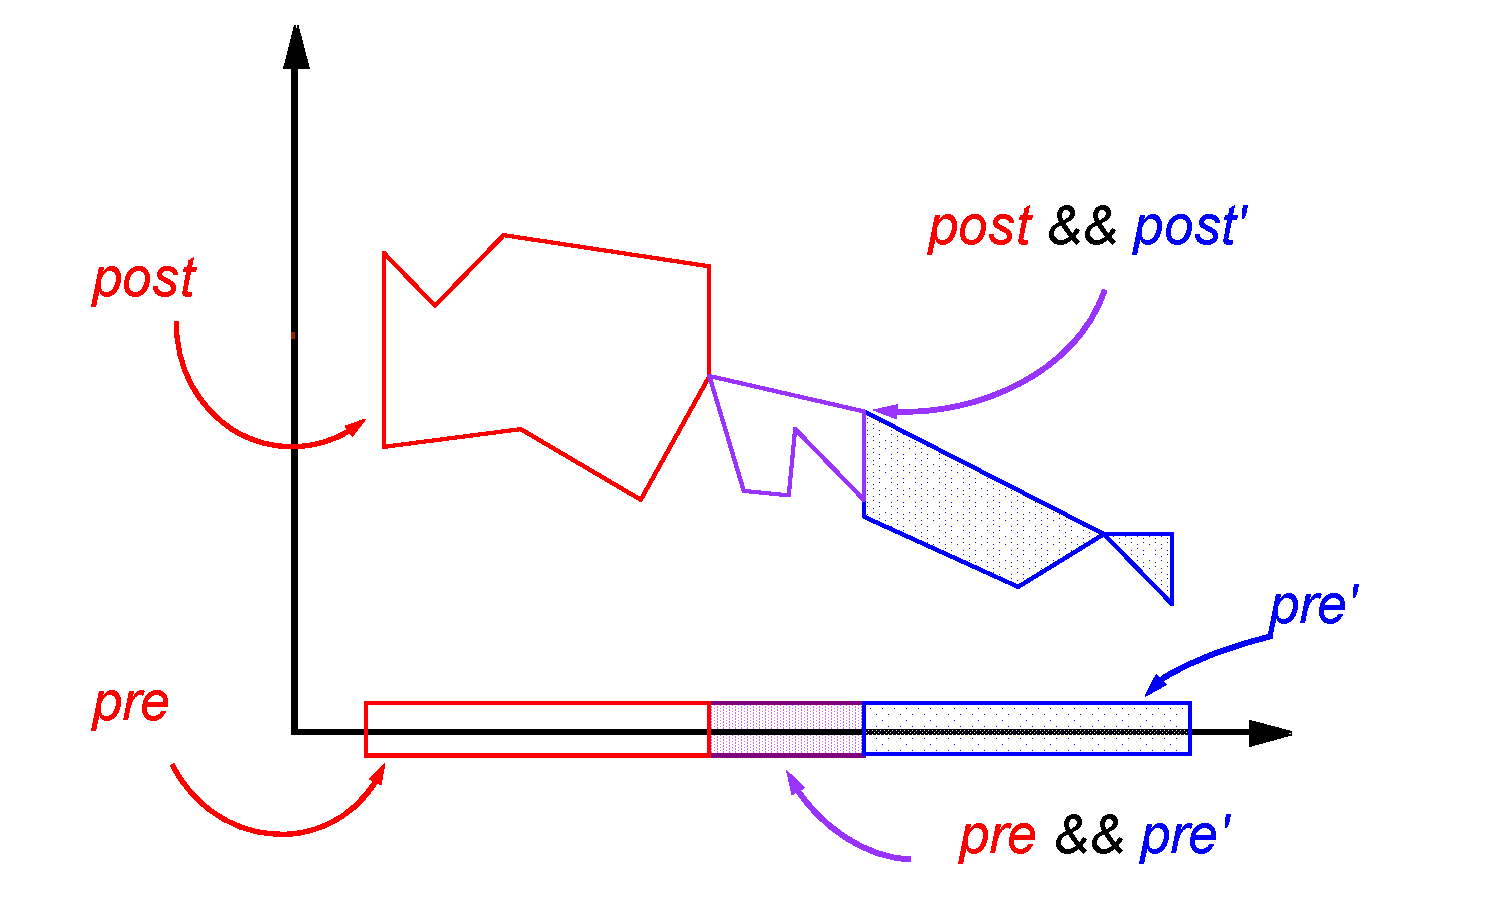
\includegraphics[width=4.25in]{join-intersect}
\end{frame}

\begin{frame}[fragile]
\frametitle{Meaning of 'also'}
\begin{lstlisting}
  requires 0 <= a && a <= 150;
  assignable age;
  ensures age == a;
also
  requires a < 0;
  assignable \nothing
  ensures age == \old(age);
\end{lstlisting}
\end{frame}

\begin{frame}[fragile]
\frametitle{Meaning of `also'}
\begin{lstlisting}
  requires 0 <= a && a <= 150;
  assignable age;
  ensures age == a;
also
  requires a < 0;
  assignable age;
  ensures age == \old(age)
      && \only_assigned(\nothing);
\end{lstlisting}
\note{Can only join where the frames are the same.}
\end{frame}

\begin{frame}[fragile]
\frametitle{Meaning of `also'}

\begin{lstlisting}
  requires (0 <= a && a <= 150) || a < 0;
  assignable age;
  ensures \old(0 <= a && a <= 150)
       ==> (age == a);
  ensures \old(a < 0)
       ==> (age == \old(age)
            && \only_assigned(\nothing));
\end{lstlisting}
\note{The original is easier to read than this desugared version,
      which is the point of having multiple cases.
      This last version could of course be simplified a bit.
}
\end{frame}

\begin{frame}[fragile]
\frametitle{Notation for Method Specification in $T$}

\begin{lstlisting}[mathescape=true]
  public interface $T$ {
    //@ requires $\pre$;
    //@ ensures $\post$;
    void m();
  }
\end{lstlisting}

~

$T \At (\pre, \post)$
\end{frame}


\begin{frame}
\frametitle{Join of Specification Cases, $\join^{S}$}
\begin{definition}
If \BLUE{${T' \At (\pre',\post')}$}, \RED{$T \At (\pre, \post)$},
$S \STO \BLUE{T'}$, $S \STO \RED{T}$, 
then
\begin{displaymath}
\BLUE{(\pre',\post')} \:\join^S\: \RED{(\pre,\post)} = (p,q)
\end{displaymath}
where $p = \BLUE{\pre'} \mbox{\texttt{ || }} \RED{\pre}$ \\
and $q = (\texttt{\textbackslash\textbf{old}(}\BLUE{\pre'}\texttt{)}
   \mbox{\texttt{ ==> }} \BLUE{\post'})
\mbox{\texttt{ \&\& }}
  (\texttt{\textbackslash\textbf{old}(}\RED{\pre}\texttt{)}
   \mbox{\texttt{ ==> }} \RED{\post})$ \\
and $S \At (p, q)$.
\end{definition}
\end{frame}


\begin{frame}
\frametitle{Client's View of Multiple Cases}

Client can verify by:
\begin{itemize}
\item
Picking one spec case.
\begin{itemize}
\item
Assert precondition.

\item
Assume frame and postcondition.
\end{itemize}

\item
Picking several cases.
\begin{itemize}
\item
Compute their join.

\item
Assert joined precondition.

\item
Assume frame and joined postcondition.
\end{itemize}
\end{itemize}
\note{Conditions must be adapted to the actual parameters by substitution...

Computing the join is easy if the preconditions are equal.
}
\end{frame}

\begin{frame}
\frametitle{Implementor's View of Multiple Cases}

\begin{itemize}
\item
Verify each case, or

\item
Verify their join.
\end{itemize}
\note{Assume each precondition and assert each postcondition,
or assume the disjunction of the preconditions, and verify the
conjunction of implications.
}
\end{frame}


\begin{frame}
\frametitle{Background for Specifying Exceptions}

Java Exceptions:
\begin{itemize}
\item
Unchecked (RuntimeException):
\begin{itemize}
\item
Client avoidable (use preconditions).

\item
Implementation faults (fix them).
\end{itemize}

\item
Checked:
\begin{itemize}
\item
Clients can't avoid (efficiently).

\item
Condition simultaneous with use (permissions).

\item
Alternative returns (not found, EOF, $\ldots$).
\end{itemize}
\end{itemize}

\end{frame}

\begin{frame}
\frametitle{When to Specify Exceptions}

Unchecked exceptions:
\begin{itemize}
\item
Don't specify them.

\item
Just specify the normal cases.
\end{itemize}

Checked exceptions
\begin{itemize}
\item
Specify them.
\end{itemize}
\end{frame}

\begin{frame}[fragile]
\frametitle{JML Features for Exception Specification}

\begin{itemize}
\item
\lstinline!exceptional_behavior! spec cases.

\item
\lstinline!signals_only! clause.

\item
\lstinline!signals! clause.
\end{itemize}
\end{frame}

\begin{frame}[fragile]
\frametitle{Exceptional Specification Example}
\lstinputlisting[linerange={1-6}]{examples/Actor.java}
\end{frame}

\begin{frame}[fragile]
\frametitle{Exceptional Specification Example}
\lstinputlisting[linerange={8-21}]{examples/Actor.java}
\end{frame}

\begin{frame}
\frametitle{Underspecification of Exceptions}
\begin{question}
How would you specify this, \\
ignoring the exceptional behavior? 
\end{question}
\note{That is, how to write the specification and ignore the
  exceptional case?
}
\end{frame}

\begin{frame}<beamer>
\frametitle{Underspecification of Exceptions}
\lstinputlisting[linerange={8-14}]{examples/ActorUnderspecified.java}
\end{frame}


\begin{frame}[fragile]
\frametitle{Heavyweight Behavior Spec Cases}
\framesubtitle{Presumed Complete}

\lstinline!normal_behavior!, \lstinline!exceptional_behavior!
\begin{itemize}
\item
Say how method can terminate.

\item
Maximally permissive/useless defaults.
\end{itemize}

\lstinline!behavior!
\begin{itemize}
\item
Doesn't specify normal/exceptional.

\item
Can use to underspecify normal/exceptional.
\end{itemize}
\note{Generally, the defaults for boolean clauses are ``true''.

But for frames (assignable) the default is
\texttt{\textbackslash}\lstinline!everything!, 
as that is most permissive.

However, \lstinline!signals_only! has a default that is based on the
declared exceptions in a method (see below).
}
\end{frame}

\begin{frame}[fragile]
\frametitle{Lightweight Specification Cases}
\framesubtitle{Presumed Incomplete}

\begin{itemize}
\item
Don't use a behavior keyword.

\item
Most defaults technically \lstinline!\not_specified!.
\end{itemize}
\end{frame}

\begin{frame}[fragile]
\frametitle{Semantics of signals\_only}

\begin{itemize}
\item
\lstinline!signals_only! $T_1, \ldots, T_n$\texttt{;}
\begin{itemize}
\item
Exception thrown to caller must subtype
one $T_1, \ldots, T_n$.
\end{itemize}

\item
Can't use in \lstinline!normal_behavior!

\item
At most one \lstinline!signals_only! clause per spec case.

\item
Default for omitted clause
\begin{itemize}
\item
if method declares \lstinline!throws! $T_1, \ldots, T_n$,
\newline
then \lstinline!signals_only! $T_1, \ldots, T_n$\texttt{;}.

\item
else \lstinline!signals_only \nothing;!.
\end{itemize}
\end{itemize}
\note{Assuming $n > 0$.
  The default only applies to lightweight spec cases and
  heavyweight \lstinline!exceptional_behavior! spec cases.
}
\end{frame}

\begin{frame}
\frametitle{Signals Clause}

\begin{itemize}
\item
Specifies, when exception thrown,
\begin{itemize}
\item
State of exception object.

\item
Other state.
\end{itemize}

\item
Not very useful.

\item
Tip: normally omit.
\end{itemize}
\end{frame}

\begin{frame}
\frametitle{Pitfalls in Exceptional Specification}
\begin{itemize}
\item
Can't return normally \emph{and\/} throw exception.

\item
So preconditions shouldn't overlap.
\end{itemize}

\begin{question}
What happens if they overlap?
\end{question}
\note{The specification will be unsatisfiable (for the overlap).

  In many such cases you want to use a single Behavior.
  See \texttt{examples/Factor.java} for how to do this.
}
\end{frame}

\begin{frame}
\frametitle{Exercise Using Multiple Cases}

\begin{exercise}
Specify the $3x+1$ or ``hailstone'' function, $h$,
such that:

\begin{displaymath}
h(n) = 
\left\{
\begin{array}{ll}
(3 \times n + 1)/2, & \mbox{if $n>0$ is odd} \\
n / 2,              & \mbox{if $n>0$ is even}
\end{array}
\right.
\end{displaymath}

and $h$ is undefined on negative numbers.
\end{exercise}
\end{frame}

\begin{frame}[fragile]
\frametitle{My Answer}
\lstinputlisting[linerange={3-11}]{examples/Hailstone2.java}
\end{frame}

\begin{frame}[fragile]
\frametitle{My Answer, Using Nesting}
\lstinputlisting[linerange={3-11}]{examples/Hailstone.java}
\note{Explain the nesting of spec cases by conjoining the outer
  requires onto each inner requires.  That is, it's sugar for the
  previous slide.

  Why not specify an exception?  Because the user can control the
  argument, so best just to have a precondition.
}
\end{frame}


%\part{Advanced JML}

\section[Abstr.]{Abstraction in Specification}

\subsection[Motivation]{Motivation and Overview}

\begin{frame}
\frametitle{Abstraction in Specification}

Why use abstraction?
\begin{itemize}
\item
Ease maintenance by information hiding.

\item
Readability:
\begin{itemize}
\item
Avoid quantifiers.

\item
Repeated expressions.
\end{itemize}

\item
Specify when no fields available \\
Java \textbf{\texttt{interface}}s.
\end{itemize}
\end{frame}

\begin{frame}[fragile]
\frametitle{Features Supporting Abstraction}

\begin{itemize}
\item
\lstinline!model! fields and \lstinline!represents! clauses.

\item
\lstinline!pure model! methods.

\item
\lstinline!pure! methods.

\item
\lstinline!protected! invariants, spec cases, etc.

\item
\lstinline!private! invariants, spec cases, etc.
\end{itemize}
\end{frame}

\subsection[Views]{Views of Specifications}

\begin{frame}
\frametitle{Kinds of Clients}
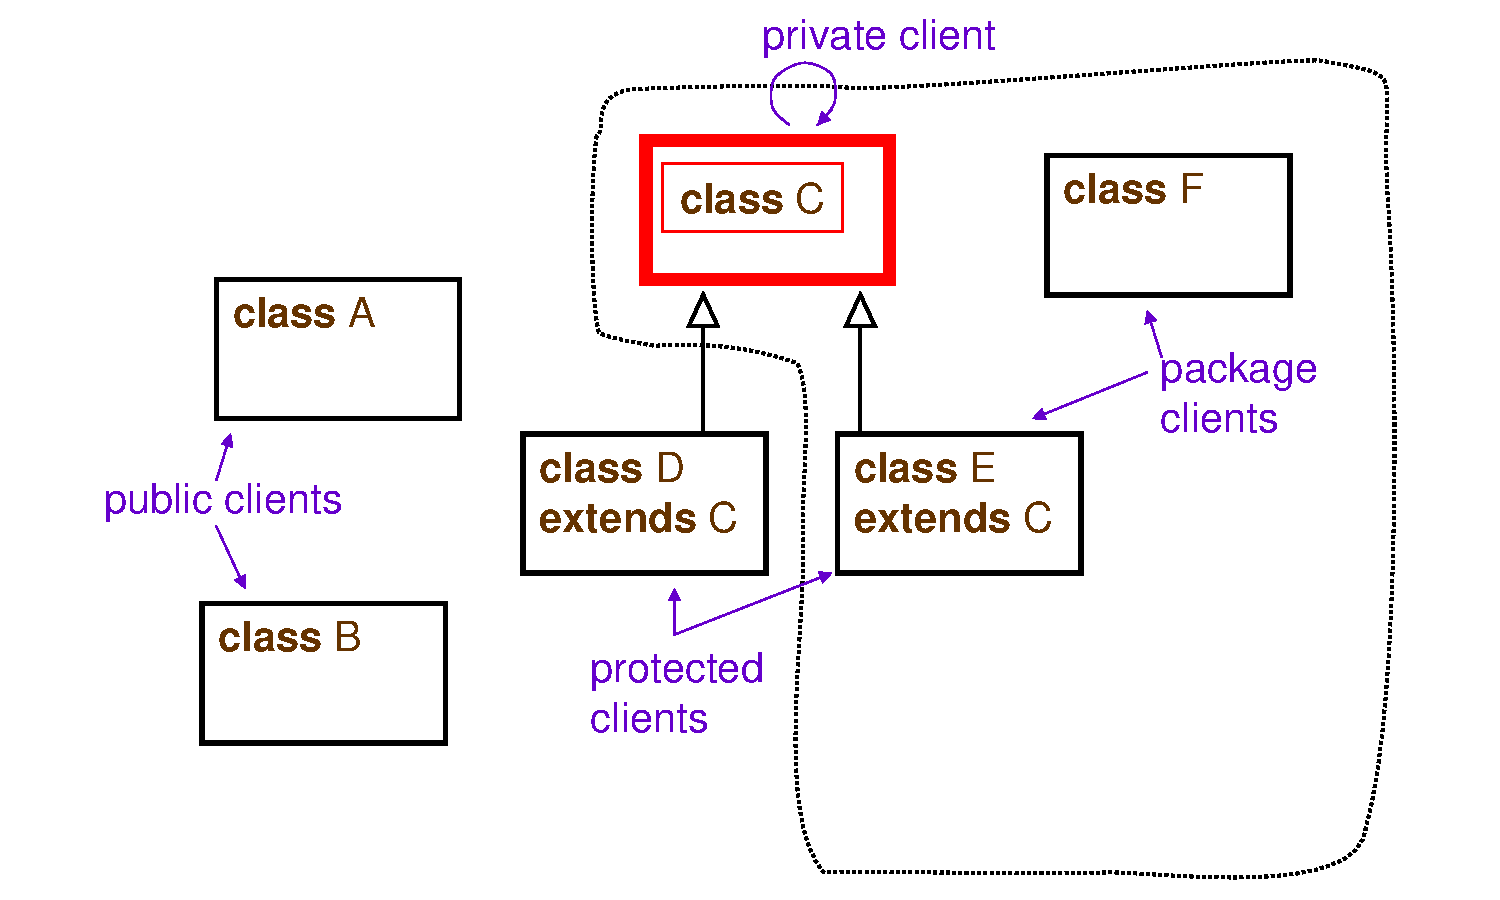
\includegraphics[width=4.25in]{visibility-modifiers}
\note{The public clients are all most specification languages discuss.

  This and some other parts on visibility and information hiding
  are from work by Leavens and Mueller presented at ICSE 2007.
}
\end{frame}

\begin{frame}
\frametitle{Views of Specifications}
\begin{tabular}{ll}
         & Declarations in $C$ \\
Modifier & visible to code in: \\
\hline
Private          & $C$ \\
(None = package) & $C$'s package \\
Protected        & $C$'s subclasses, \\
                 & $C$'s package \\
Public           & all
\end{tabular}
\note{ESC/Java2 currently ignores some of the visibility checks.

But it is checked by other JML tools, and should be checked eventually
by ESC/Java2 also.
}
\end{frame}

\begin{frame}
\frametitle{Privacy and Modular Soundness}
Specifications visible to module $M$:
\begin{itemize}
\item
Can only mention members visible to $M$.
\begin{itemize}
\item
For maintenance.

\item
For understandability.
\end{itemize}

\item
Must contain all of $M$'s obligations.
\begin{itemize}
\item
For sound modular verification.
\end{itemize}
\end{itemize}
\end{frame}

\begin{frame}
\frametitle{Privacy and Modular Soundness}
\begin{question}
Can private fields be mentioned in public specifications?
\end{question}
\note<1>{No, it volates the principles given.}

\pause
\begin{question}
Can non-trivial preconditions be hidden from clients?
\end{question}
\note<2>{No, it volates the principles given.}

\pause
\begin{question}
What should a client assume is the precondition of \\
a method with no visible specification cases?
\end{question}
\note<3>{The predicate ``true''.}

\pause
\begin{question}
If invariant $\inv$ depends on field $f$, \\
can $\inv$ be less visible than $f$?
\end{question}
\note<4>{No, it volates the principles given.}
\end{frame}

\subsection[Model]{Data Abstraction with Model Fields}

\begin{frame}[fragile]
\frametitle{Model Fields for Data Abstraction}

Model fields:
\begin{itemize}
\item
Just for specification.

\item
Abstraction of Java fields.

\item
Value from \lstinline!represents!.
\end{itemize}
\end{frame}

\begin{frame}[fragile]
\frametitle{Model Field in an Interface}
\lstinputlisting{examples/Gendered.java}
\note{We use \lstinline!instance! because by default fields in Java
  interfaces are static.}
\end{frame}

\begin{frame}[fragile]
\frametitle{Represents Clauses}
\lstinputlisting[linerange={1-5,16-19}]{examples/Animal.java}
\end{frame}

\begin{frame}
\frametitle{Correctness with Model Fields}
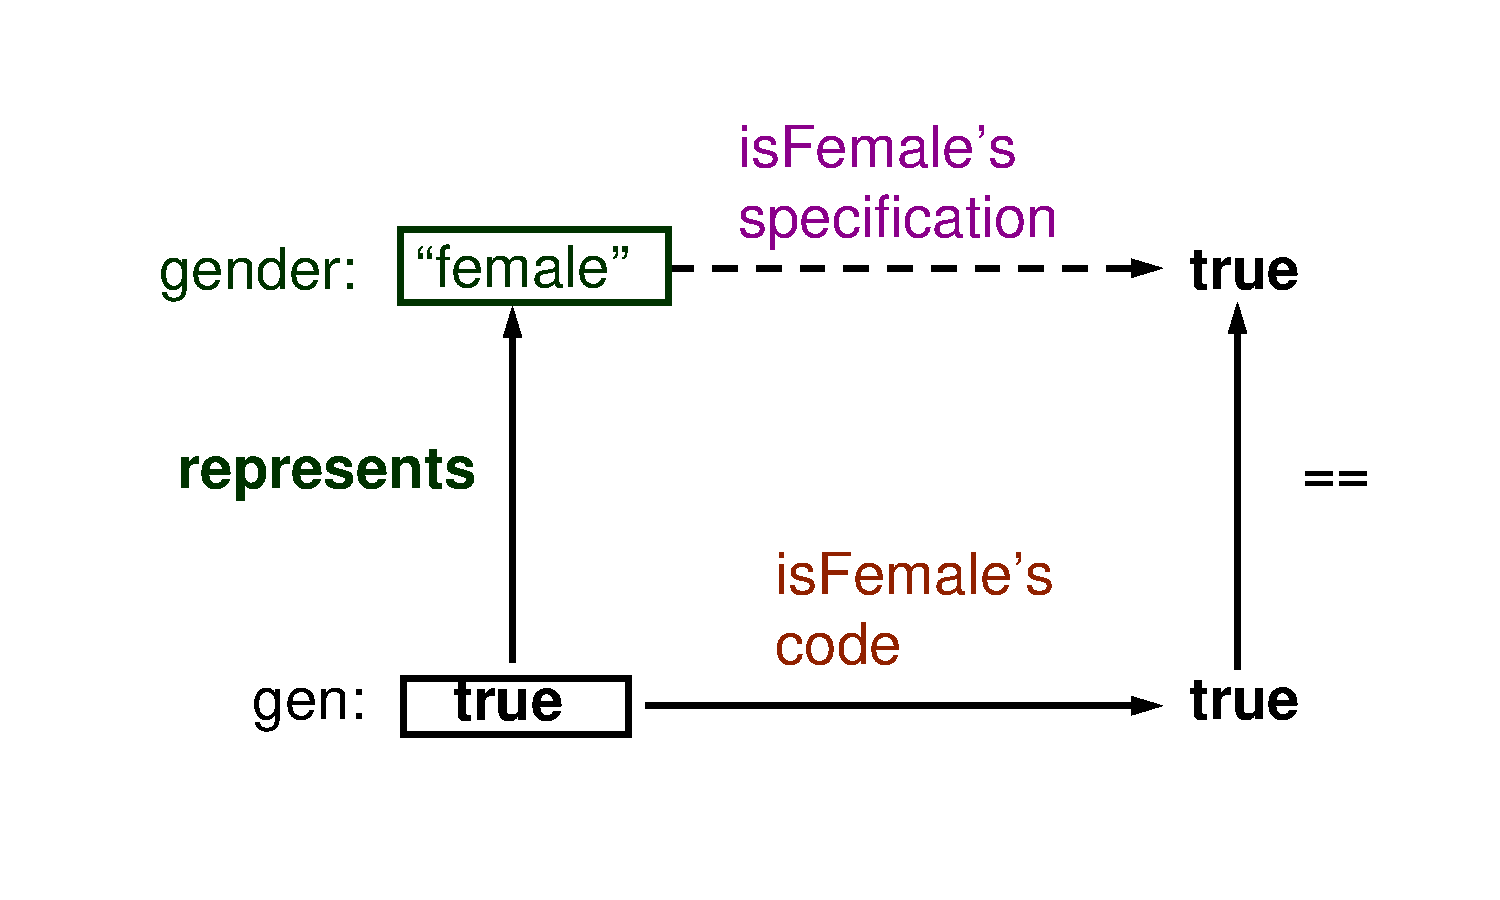
\includegraphics[width=4.25in]{model-correctness}
\end{frame}

\begin{frame}[fragile]
\frametitle{Example of Using Model Fields}
\begin{question}
Is Animal's constructor (below) correct?
\rm
\lstinputlisting[linerange={2-5,8-14}]{examples/Animal.java}
\end{question}
\end{frame}

\begin{frame}<beamer>[fragile]
\frametitle{Example of Using Model Fields}

\alert{Yes!}

\lstinputlisting[linerange={2-5,8-14}]{examples/Animal.java}

\end{frame}

\begin{frame}[fragile]
\frametitle{Semantics of \lstinline!spec_public!}
\lstinputlisting[linerange={7-7}]{examples/Animal.java}

shorthand for:

\begin{lstlisting}
  //@ public model int age;
  //@ protected int _age = 0; //@ in age;
  //@ protected represents age <- _age; 
\end{lstlisting}

and rewriting Java code to use \lstinline!_age!.

\note{Can use this for changing \lstinline!spec_public! declarations.}
\end{frame}

\begin{frame}
\frametitle{Data Groups for Assignable Clauses}
\begin{itemize}
\item
Each field is a data group.

\item
Membership by \JMLKW{in} clauses.

\item
Model field's group contains
fields used in its \JMLKW{represents}.
\end{itemize}
\end{frame}

\begin{frame}
\frametitle{Data Groups and Assignable Picture}
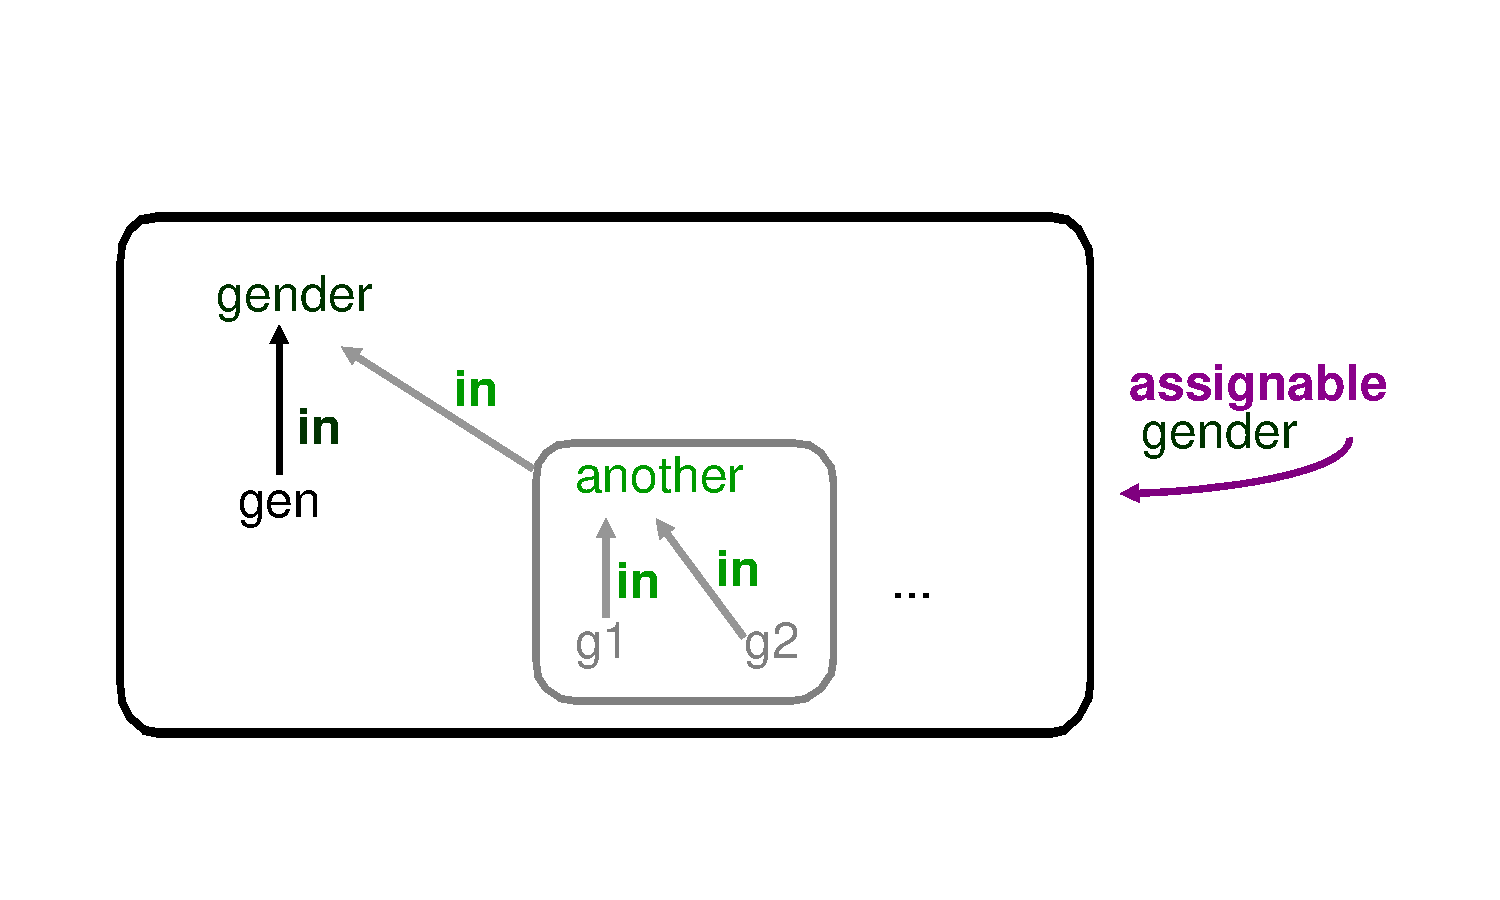
\includegraphics[width=4.25in]{datagroup}
\end{frame}

\begin{frame}[fragile]
\frametitle{The Semantics of Assignable}

\lstinline!assignable! $x$, $y$\texttt{;}

~~means:

method only assigns to (concrete) members of 
$\DG(x) \cup \DG(y)$.

\begin{question}
What does \lstinline!assignable gender;! mean?
\end{question}
\note{We use $\DG(x)$ in this talk as the data group of $x$.
The method only assigns to gen or other members of gender's data group.
}
\end{frame}

\begin{frame}[fragile]
\frametitle{In Clauses for Declarations}

\lstinline!private! $T$ $x$\lstinline!; //@ in! $g$\texttt{;}

\begin{itemize}
\item
Immediately follows declaration

\item
Same visibility as declaration.
\end{itemize}

JML ensures that:
\begin{itemize}
\item
If $f \in \DG(g)$, then $g$ visible where $f$ is.

\item
If $f$ and $g$ visible,
can tell if $f \in \DG(g)$.
\end{itemize}
\note{The first of these is Leino and Nelson's (2002) Authenticity rule.}
\end{frame}

\begin{frame}[fragile]
\frametitle{Data Group Visibility and Reasoning}

\begin{question}
Can assigning to \lstinline!age! change \lstinline!gender!?
\end{question}
\note{No, we can tell they are in distinct data groups, since we've
  seen both declarations and they aren't connected.
  JML makes sure that we can't put age in gender's data group later.
}
\end{frame}

\subsection[Advanced]{Advanced Data Abstraction}

\begin{frame}[fragile]
\frametitle{Type-Level Specification Features}

\begin{itemize}
\item
fields, \lstinline!in!, \lstinline!represents!

\item
\lstinline!invariant!

\item
\lstinline!initially!

\item
\lstinline!constraint!
\end{itemize}
\end{frame}

\begin{frame}[fragile]
\frametitle{Initially Clauses}

\begin{itemize}
\item
Hold in constructor post-states.

\item
Basis for datatype induction.
\end{itemize}

\lstinputlisting[linerange={1-6}]{examples/Patient.java}

\end{frame}

\begin{frame}
\frametitle{History Constraints}
\begin{itemize}
\item
Relate pre-states and post-states.

\item
Justifies inductive step in datatype induction.
\end{itemize}
\end{frame}

\begin{frame}[fragile]
\frametitle{History Constraints}
\lstinputlisting[linerange={1-2}]{examples/Patient.java}
\lstinputlisting[linerange={5-5}]{examples/Patient.java}
\lstinputlisting[linerange={10-15}]{examples/Patient.java}
\end{frame}

\subsection[Other]{Other Topics}

\begin{frame}[fragile]
\frametitle{Helper Methods and Constructors}

A \lstinline!helper! method or constructor is:
\begin{itemize}
\item
\lstinline!private!

\item
Exempt from invariants and history constraints.
\begin{itemize}
\item
Cannot assume them.

\item
Need not establish them.
\end{itemize}
\end{itemize}

\note{By default \lstinline!private! methods must preserve invariants
and history constraints.  Have to label them \lstinline!helper! if
don't want that.
}
\end{frame}

\begin{frame}[fragile]
\frametitle{Ghost fields and Local Variables}
\begin{itemize}
\item
Specification-only data.

\item
No \lstinline!represents! clause.

\item
Value from initialization and \lstinline!set! statements.

\item
Locals useful for loop invariants, termination, etc.
\end{itemize}
\end{frame}

\begin{frame}[fragile]
\frametitle{Owner is a Ghost Field}

Declaration:

\begin{lstlisting}
public class Object {
  //@ public ghost Object owner = null;
  /* ... */
}
\end{lstlisting}

Assignment:
\begin{lstlisting}
  //@ set a.owner = this;
\end{lstlisting}
\end{frame}

\section[Subtypes]{Subtyping and Specification Inheritance}

\begin{frame}
\frametitle{Problems}
\begin{itemize}
\item
Duplication of specifications in subtypes.

\item
Modular verification when use:
\begin{itemize}
\item
Subtyping, and

\item
Dynamic dispatch.
\end{itemize}
\end{itemize}
\end{frame}

\subsection[Spec. Inh.]{Specification Inheritance}

\begin{frame}
\frametitle{Specification Inheritance Approach}

Inherit:
\begin{itemize}
\item
Instance fields.

\item
Type specifications.

\item
Instance methods.

\item
Method specification cases.
\end{itemize}
\end{frame}

\begin{frame}
\frametitle{Multiple Inheritance Example}
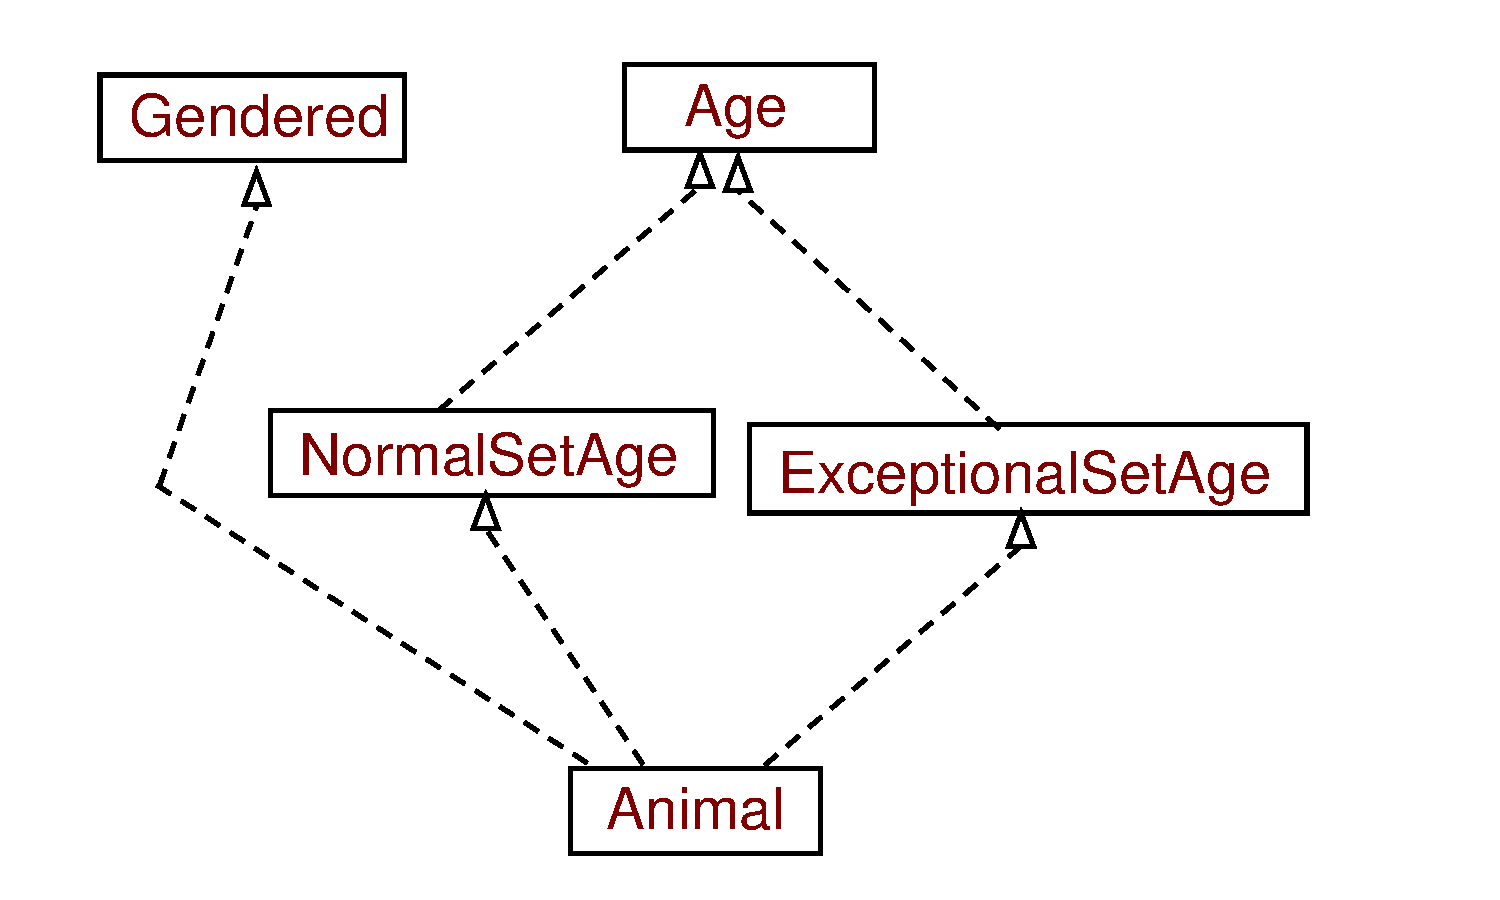
\includegraphics[width=4.25in]{multiple-inh}
\end{frame}

\begin{frame}[fragile]
\frametitle{Age and NormalSetAge}
\begin{lstlisting}
public interface Age {
  //@ model instance int age;
}

public interface NormalSetAge 
           implements Age {
  /*@ requires 0 <= a && a <= 150;
    @ assignable age;
    @ ensures age == a;   @*/
  public void setAge(int a);
}
\end{lstlisting}
\end{frame}

\begin{frame}[fragile]
\frametitle{ExceptionalSetAge}
\begin{lstlisting}
public interface ExceptionalSetAge
           implements Age {
  /*@ requires a < 0;
    @ assignable \nothing;
    @ ensures age == \old(age);   @*/
  public void setAge(int a);
}
\end{lstlisting}
\end{frame}

\begin{frame}
\frametitle{What About Animal's setAge method?}

\begin{itemize}
\item
It's both.

\item
Should \alert{obey both specifications}.
\end{itemize}
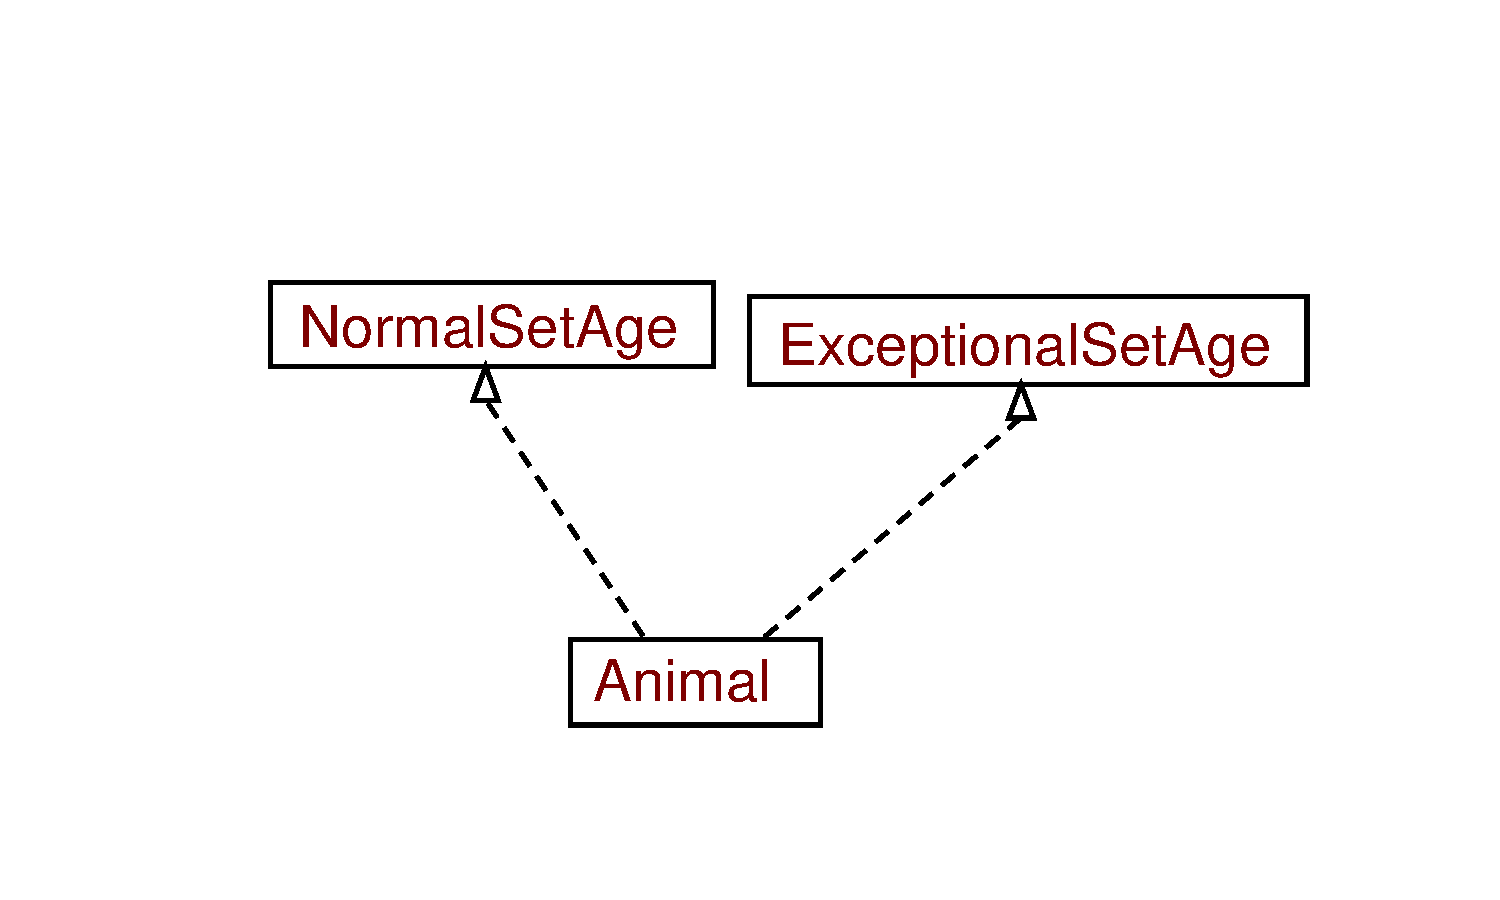
\includegraphics[height=2in]{multiple-inh2}
\end{frame}

\begin{frame}[fragile]
\frametitle{Single Inheritance also}
\begin{question}
What is the specification of Animal's \texttt{isFemale} method?

\rm
\lstinputlisting[linerange={1-1,4-6}]{examples/Gendered.java}

\lstinputlisting[linerange={1-1,15-18,29-29}]{examples/Animal.java}
\end{question}
\note{The one inherited from Gendered.}
\end{frame}

\begin{frame}[fragile]
\frametitle{Adding to Specification in Subtype}
\framesubtitle{Use of `also' Mandatory}

\lstinputlisting[linerange={1-2,31-40}]{examples/Patient.java}
\end{frame}

\begin{frame}
\frametitle{Method Specification Inheritance}

\begin{question}
What is the extended specification of \texttt{Patient}'s
\texttt{setAge} method?
\end{question}
\note{The join of the 3 spec cases shown previously}
\end{frame}

\begin{frame}[fragile]
\frametitle{Extended Specification of SetAge}
\lstinputlisting[linerange={20-26}]{examples/Animal.java}
\lstinputlisting[linerange={34-36}]{examples/Patient.java}
\end{frame}

\begin{frame}[fragile]
\frametitle{Avoiding Duplication of Preconditions}
\lstinputlisting[linerange={20-26}]{examples/Animal.java}
\begin{lstlisting}
  /*@ also
    @   requires \same;
    @   ensures 65 <= age ==> ageDiscount;  @*/
\end{lstlisting}
\note{The \texttt{\textbackslash}\lstinline!same! in the requires clause
doesn't yet work in ESC/Java2.}
\end{frame}

\begin{frame}
\frametitle{Method Specification Inheritance}
\begin{question}
In JML, can you override a method \\
and make its precondition more restrictive?
\end{question}
\note{No.  You can only use the same or weaker precondition.  If you
  think you're strengthening it, you actually are just describing a
  special case.
}
\end{frame}

\begin{frame}<beamer>[fragile]
\frametitle{No, You Can't Strengthen Preconditions}
\framesubtitle{Can Point Out Special Cases}
\lstinputlisting[linerange={2-2}]{examples/Person.refines-jml}

\lstinputlisting[linerange={3-7}]{examples/Person.refines-jml}
\end{frame}


\begin{frame}
\frametitle{Inheritance of Type Specifications}

Obeyed by all subtypes:
\begin{itemize}
\item
Invariants.

\item
Initially Clauses.

\item
History Constraints.
\end{itemize}
\end{frame}

\begin{frame}
\frametitle{Invariants Obeyed by Subtypes}
\framesubtitle{Not a Syntactic Sugar}
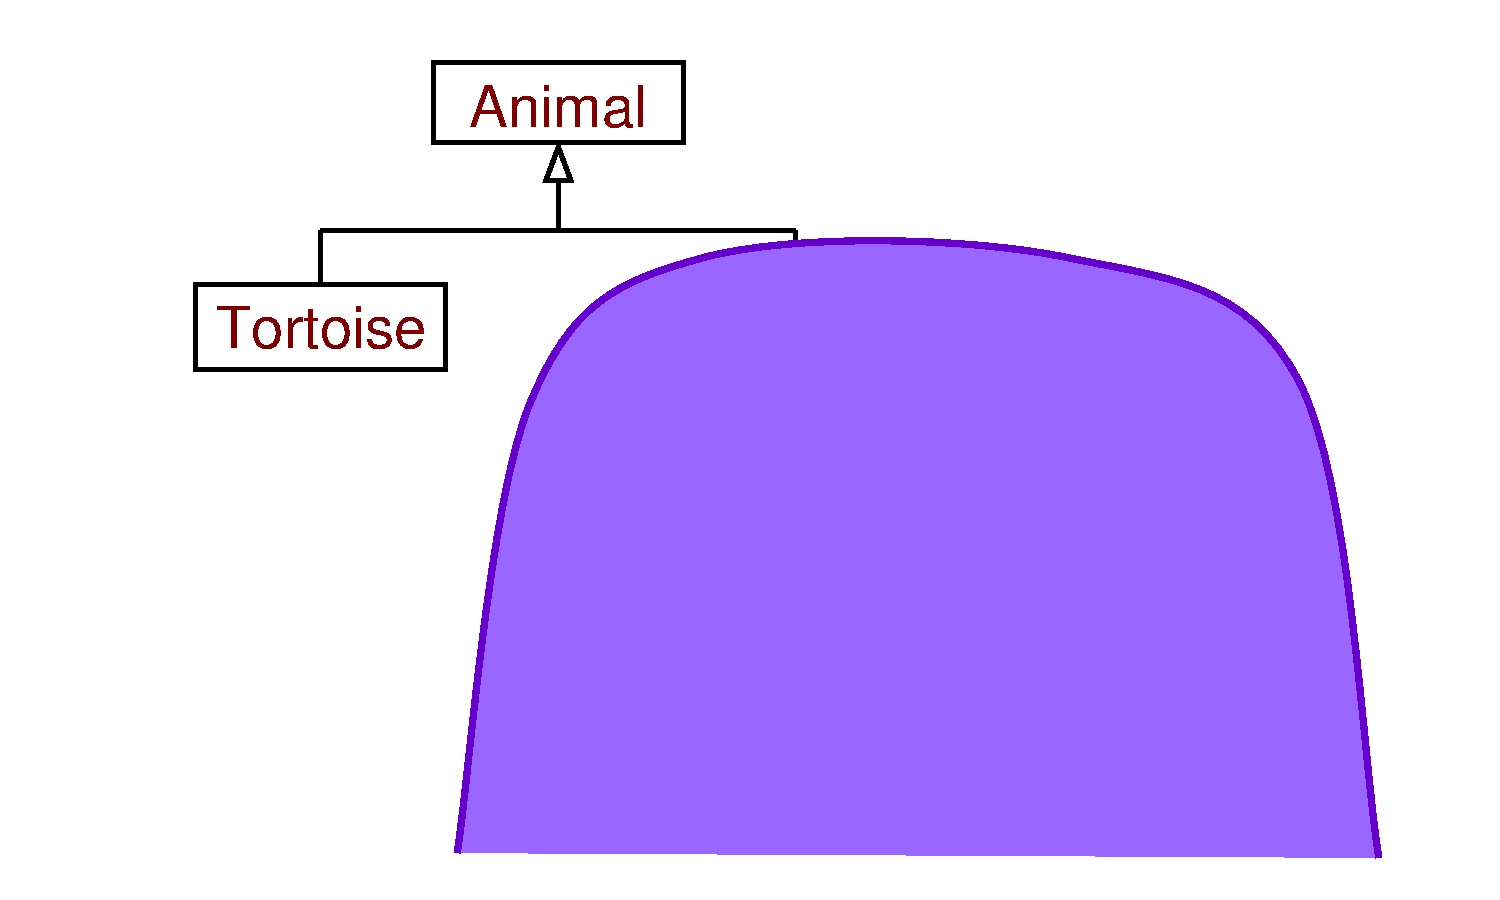
\includegraphics[width=4.25in]{invariant-inh}
\end{frame}

\begin{frame}
\frametitle{Notation for Describing Inheritance}
\framesubtitle{$T$'s Added Specification}

Declared in $T$ (without inheritance):
\begin{center}
\begin{tabular}{ll}
$\addedinv^T$ & invariant \\
$\addedhc^T$ & history constraint\\
$\addedinit^T$ & initially predicate \\
$\addedspec^T_m$ & $m$'s specification \\
\end{tabular}
\end{center}

Other Notations:
\begin{displaymath}
\supers(T) = \{U \mid T \STO U\}
\end{displaymath}
\begin{displaymath}
\methods({\cal T}) = \{m \mid m \mbox{ declared in } T \in {\cal T}\}
\end{displaymath}
\end{frame}

\begin{frame}
\frametitle{Specification Inheritance's Meaning}
\framesubtitle{Extended Specification of $T$}

\begin{description}[Constraint:]
\item[Methods:]
for all $m \in \methods(\supers(T))$
\begin{displaymath}
\extspec^T_m = \join^T \{\addedspec^U_m \mid U \in \supers(T)\}
\end{displaymath}

\item[Invariant:]
$\extinv^T = \bigwedge \{\addedinv^U \mid U \in \supers(T)\}$

\item[Constraint:]
$\exthc^T = \bigwedge \{\addedhc^U \mid U \in \supers(T)\}$

\item[Initially:]
$\extinit^T = \bigwedge \{\addedinit^U \mid U \in \supers(T)\}$
\end{description}
\end{frame}

\begin{frame}[fragile]
\frametitle{Invariant Inheritance}
\lstinputlisting[linerange={1-2}]{examples/FemalePatient.java}

Extended Invariant:

\begin{lstlisting}[mathescape=true]
  $\addedinv^{\texttt{Gendered}}$ && $\addedinv^{\texttt{Animal}}$
  && $\addedinv^{\texttt{Patient}}$
  && $\addedinv^{\texttt{FemalePatient}}$
\end{lstlisting}
\end{frame}

\begin{frame}[fragile]
\frametitle{Invariant Inheritance}
\lstinputlisting[linerange={1-2}]{examples/FemalePatient.java}

Extended Invariant:

\begin{lstlisting}[mathescape=true]
  true && true
  && 0 <= age && age <= 150
      && (\forall int i;
            0 <= i && i < log.size();
            log.get(i) instanceof rep String)
  && gender.equals("female")
\end{lstlisting}
\end{frame}

\subsection[Modularity]{Modular Verification Problem}

\begin{frame}[fragile]
\frametitle{Modular Verification Problem}

Reasoning about dynamic dispatch:

\lstinputlisting[linerange={16-20}]{examples/Females.java}

How to verify?
\begin{itemize}
\item
Avoiding case analysis for all subtypes.

\item
Reverification when add new subtypes.
\end{itemize}
\end{frame}

\begin{frame}[fragile]
\frametitle{Supertype Abstraction}

Use static type's specification.

Example:

\lstinputlisting[linerange={16-20}]{examples/Females.java}

\begin{itemize}
\item
Static type of \lstinline!e! is \lstinline!Gendered!.

\item
Use specification from \lstinline!Gendered!.
\end{itemize}
\end{frame}

\begin{frame}[fragile]
\frametitle{Static Type's Specification}

\lstinputlisting{examples/Gendered.java}
\end{frame}

\begin{frame}
\frametitle{Supertype Abstraction in General}
Use static type's specifications to reason about:
\begin{itemize}
\item
Method calls.
\item
Invariants.
\item
History constraints.
\item
Initially predicates.
\end{itemize}
\end{frame}

\begin{frame}[fragile]
\frametitle{Supertype Abstraction Summary}

\begin{lstlisting}[mathescape=true]
$\REDT$ $o$ = createNewObject();
//@ assume $o$.$\extinit^{\REDT}$ && $o$.$\extinv^{\REDT}$;

/* ... */

//@ assert $o.\extpre^{\REDT}_m$;
$o$.$m$();
//@ assume $o.\extpost^{\REDT}_m$;
//@ assume $o.\extinv^{\REDT}_m$ && $o$.$\exthc^{\REDT}$;
\end{lstlisting}
\note<1>{Here $\REDT$ is the static type of $o$, that's why all the
  assertions refer to its specification.
}
\end{frame}

\begin{frame}
\frametitle{Reasoning Without Supertype Abstraction}

Case analysis:
\begin{itemize}
\item
Case for each potential dynamic type.

\item
Can exploit dynamic type's specifications.
\end{itemize}
\note{So this isn't modular...}
\end{frame}

\begin{frame}
\frametitle{Case Analysis + Supertype Abstraction}
\begin{itemize}
\item
Use \textbf{\texttt{instanceof}} for case analysis.

\item
Downcast, use supertype abstraction.
\end{itemize}
\note{This means you can \emph{always\/} use supertype abstraction.}
\end{frame}

\begin{frame}[fragile]
\frametitle{Case Analysis + Supertype Abstraction}
\lstinputlisting[linerange={2-12}]{examples/Staff.java}
\end{frame}

\subsection[Validity]{Supertype Abstraction's Soundness}

\begin{frame}
\frametitle{Supertype Abstraction's Soundness}
Valid if:
\begin{itemize}
\item
Invariants etc. hold as needed (in pre-states), and

\item
Each subtype is a behavioral subtype.
\end{itemize}
\end{frame}

\begin{frame}
\frametitle{Assumption about Invariants}
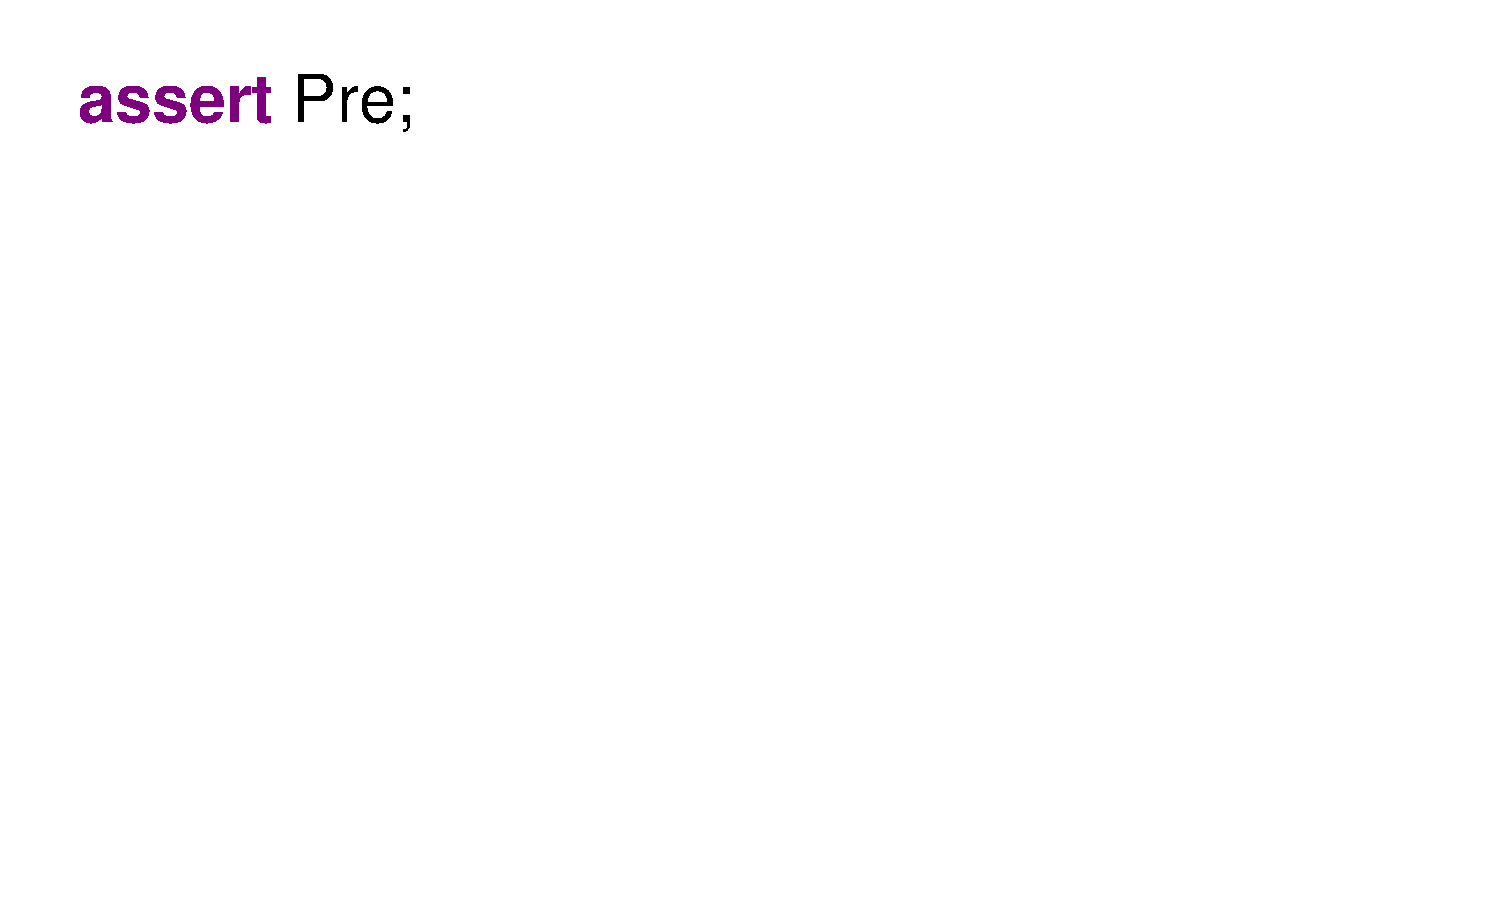
\includegraphics[width=4.25in]{invariant-call1}
\end{frame}

\begin{frame}
\frametitle{Assumption about Invariants}
\transwipe[direction=270]
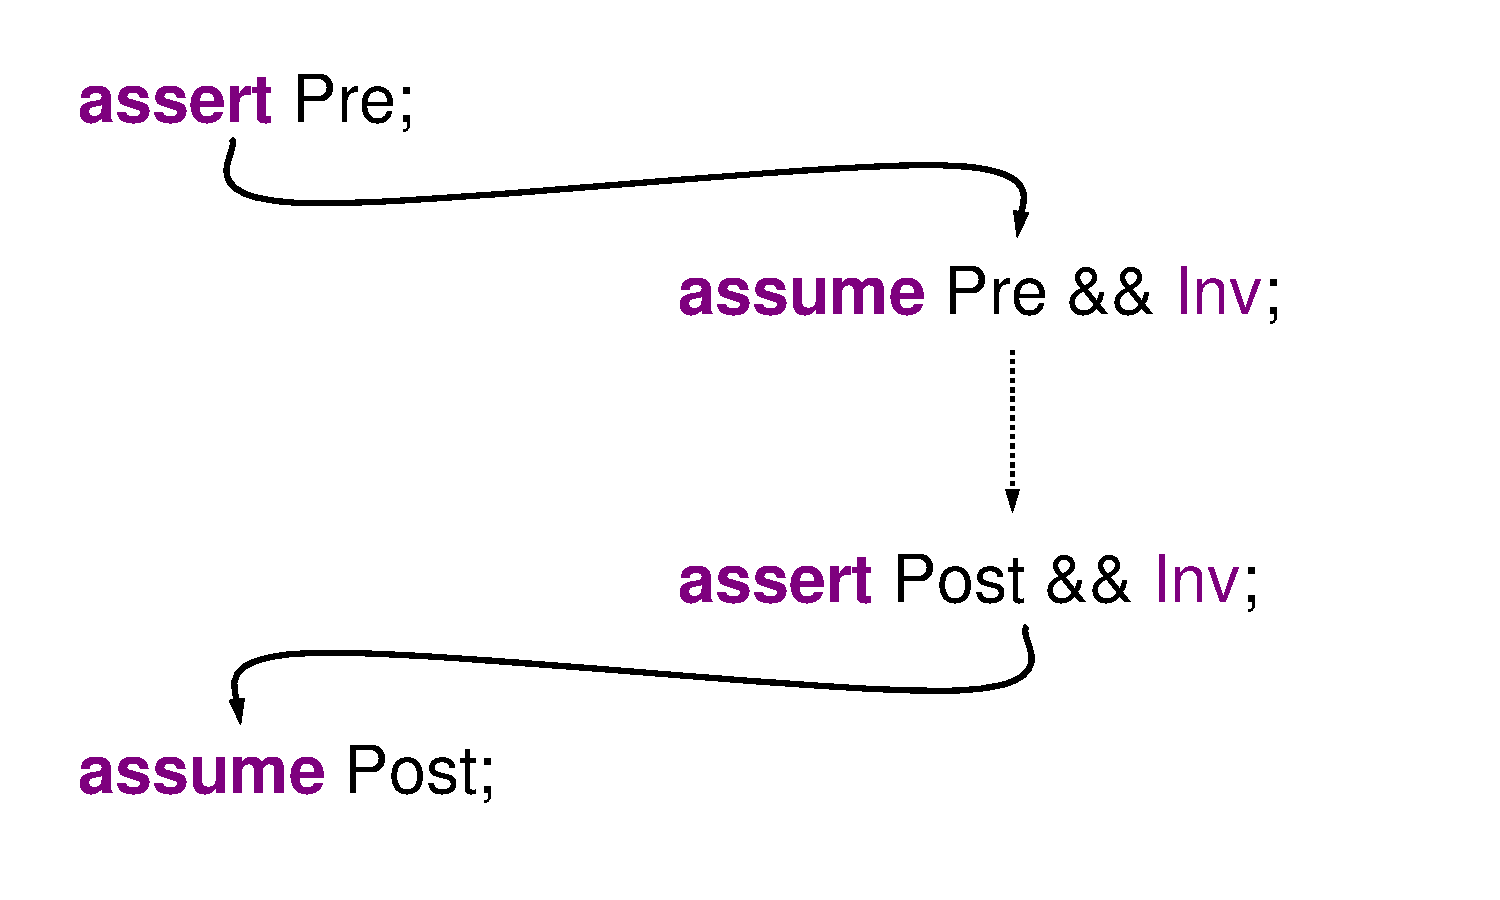
\includegraphics[width=4.25in]{invariant-call2}
\end{frame}

\begin{frame}
\frametitle{Invariant Methodology}
Potential Problems:
\begin{itemize}
\item
Representation exposure

\item
Reentrance
\end{itemize}

Relevant invariant semantics:
\begin{itemize}
\item
Ownership type system

\item
Re-establish invariant when call
\end{itemize}

Guarantees:
\begin{itemize}
\item
Invariant holds at start of method
\end{itemize}
\end{frame}

\begin{frame}
\frametitle{Open Problems}
\begin{itemize}
\item
Blending with similar Spec\# methodology.

\item
Extension to History Constraints and Initially Predicates.
\end{itemize}
\end{frame}

\begin{frame}[fragile,label=validity]
\frametitle{Validity of Supertype Abstraction}
\framesubtitle{Client's View}

\begin{lstlisting}[mathescape=true]
$\REDT$ $o$ = createNewObject();
//@ assume $o$.$\extinit^{\REDT}$ && $o$.$\extinv^{\REDT}$;

/* ... */

//@ assert $o.\extpre^{\REDT}_m$;
$o$.$m$();
//@ assume $o.\extpost^{\REDT}_m$;
//@ assume $o.\extinv^{\REDT}_m$ && $o$.$\exthc^{\REDT}$;
\end{lstlisting}
\note{Here $\REDT$ is the static type of $o$, that's why all the
  assertions refer to its specification.
}
\end{frame}

\begin{frame}[fragile]
\frametitle{What Happens at Runtime}

Suppose we have

\begin{lstlisting}[mathescape=true]
public $\REDT$ createNewObject() {
   return new $\BLUETP$();
}
\end{lstlisting}
\end{frame}

\againframe<2>{validity}

\begin{frame}[fragile]
\frametitle{Validity of Supertype Abstraction}
\framesubtitle{Implementation (Subtype) View}

\begin{lstlisting}[mathescape=true]
$\REDT$ $o$ = createNewObject(); // new $\BLUETP$()
//@ assert $o$.$\extinit^{\BLUETP}$ && $o$.$\extinv^{\BLUETP}$;

/* ... */

//@ assume $o.\extpre^{\BLUETP}_m$;
$o$.$m$();
//@ assert $o.\extpost^{\BLUETP}_m$;
//@ assert $o.\extinv^{\BLUETP}_m$ && $o$.$\exthc^{\BLUETP}$;
\end{lstlisting}
\note{Here $\REDT$ is the static type of $o$, 
     but it's dynamic type is $\BLUETP$.
}
\end{frame}

\begin{frame}
\frametitle{Behavioral Subtyping}
\begin{definition}
Suppose $\BLUETP \STO \REDT$.  Then \\
$\BLUETP$ \emph{is a strong behavioral subtype of} $\REDT$
if and only if:

\begin{itemize}
\item
for all instance methods $m$ in $\REDT$,
\begin{displaymath}
\extspec^{\BLUETP}_m \:\sqsupseteq^{\BLUETP}\: \extspec^{\REDT}_m
\end{displaymath}

\item
and whenever \textbf{\texttt{this}} has type $\BLUETP$:
\begin{displaymath}
\begin{array}{l}
\extinv^{\BLUETP} \Rightarrow \extinv^{\REDT}, \\
\exthc^{\BLUETP} \Rightarrow \exthc^{\REDT}\mbox{, and}\\
\extinit^{\BLUETP} \Rightarrow \extinit^{\REDT}.
\end{array}
\end{displaymath}
\end{itemize}
\end{definition}
\end{frame}

\begin{frame}
\frametitle{Method Specification Refinement}
\framesubtitle{With respect to $\BLUETP$}

Notation:
\begin{displaymath}
\BLUE{(\pre',\post')} \sqsupset^{\BLUETP} \RED{(\pre,\post)}
\end{displaymath}

Means:
\begin{itemize}
\item
Every correct implementation of $\BLUE{(\pre',\post')}$ satisfies
$\RED{(\pre,\post)}$.
\end{itemize}
\end{frame}

\begin{frame}
\frametitle{Method Specification Refinement}
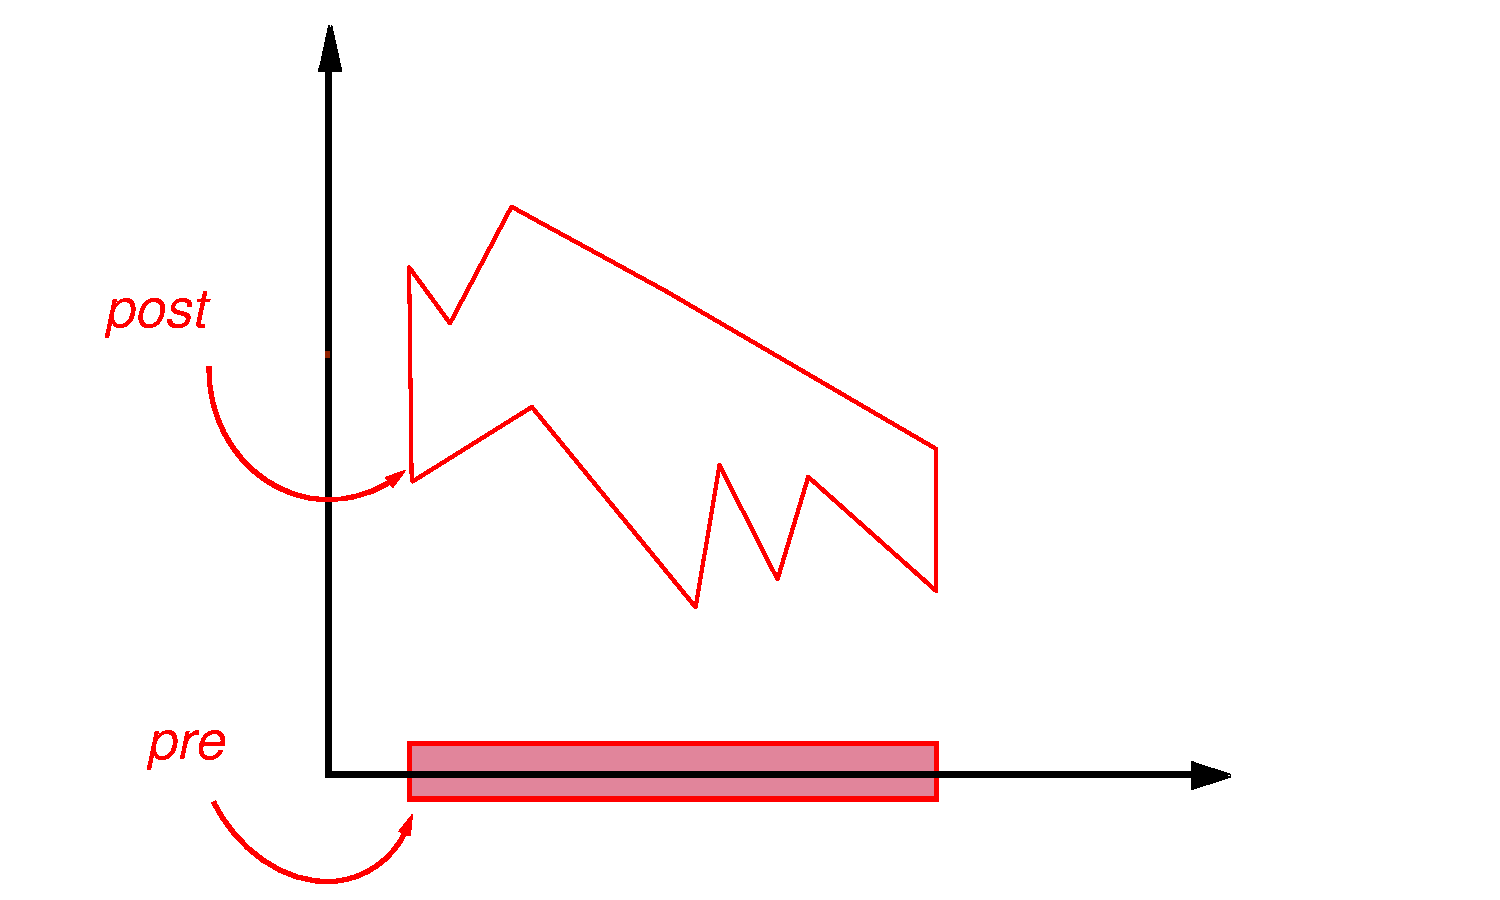
\includegraphics[width=4.25in]{meth-refine1}
\end{frame}

\begin{frame}
\frametitle{Method Specification Refinement}
\transdissolve[duration=0.2]
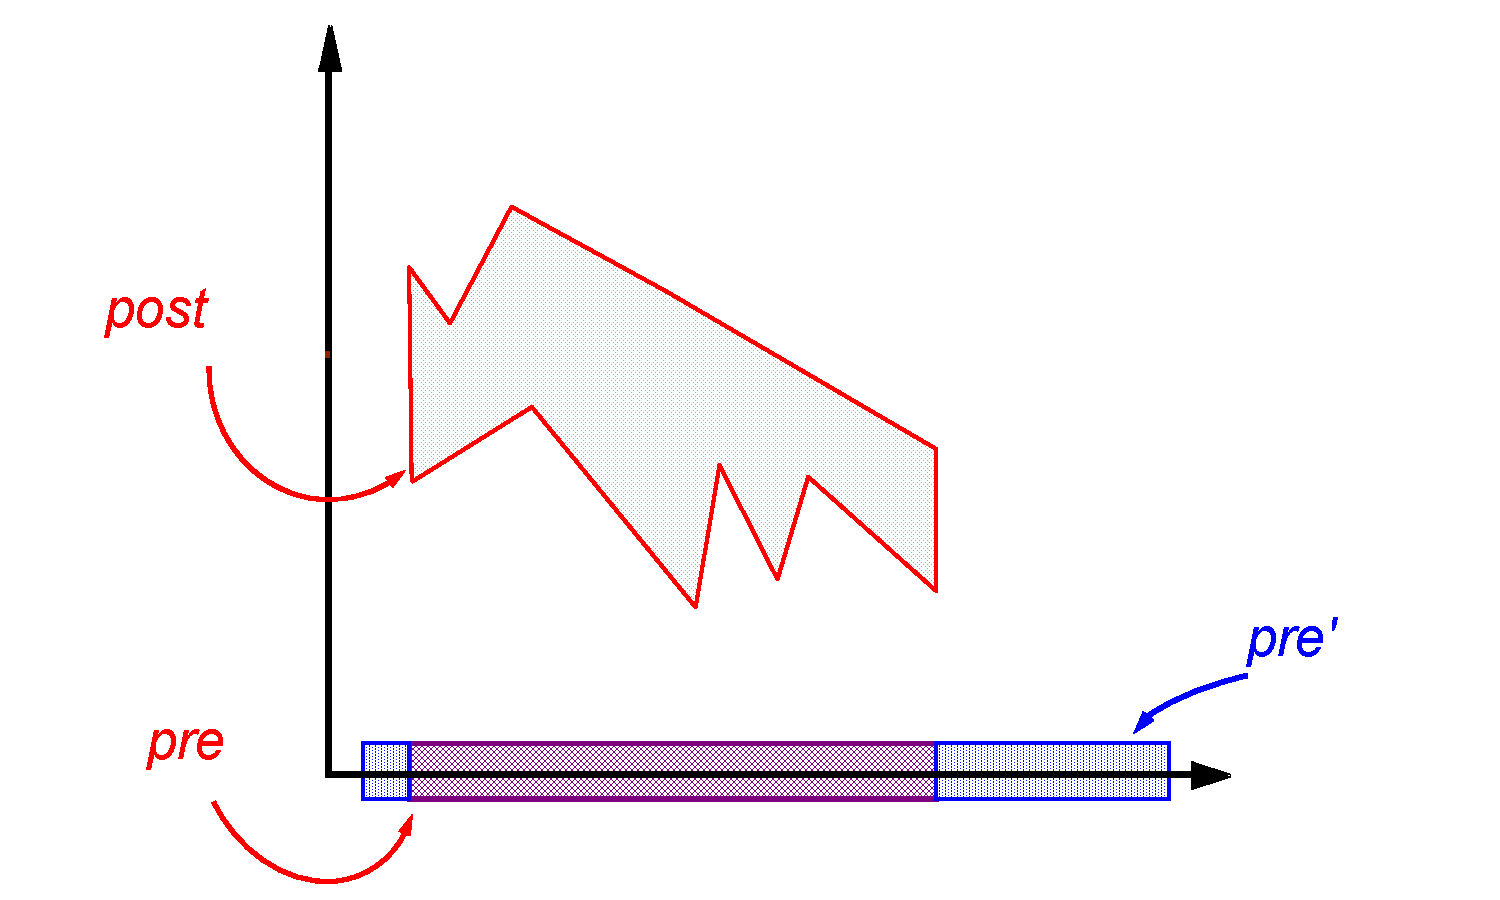
\includegraphics[width=4.25in]{meth-refine2}
\end{frame}

\begin{frame}
\frametitle{Method Specification Refinement}
\transdissolve[duration=0.2]
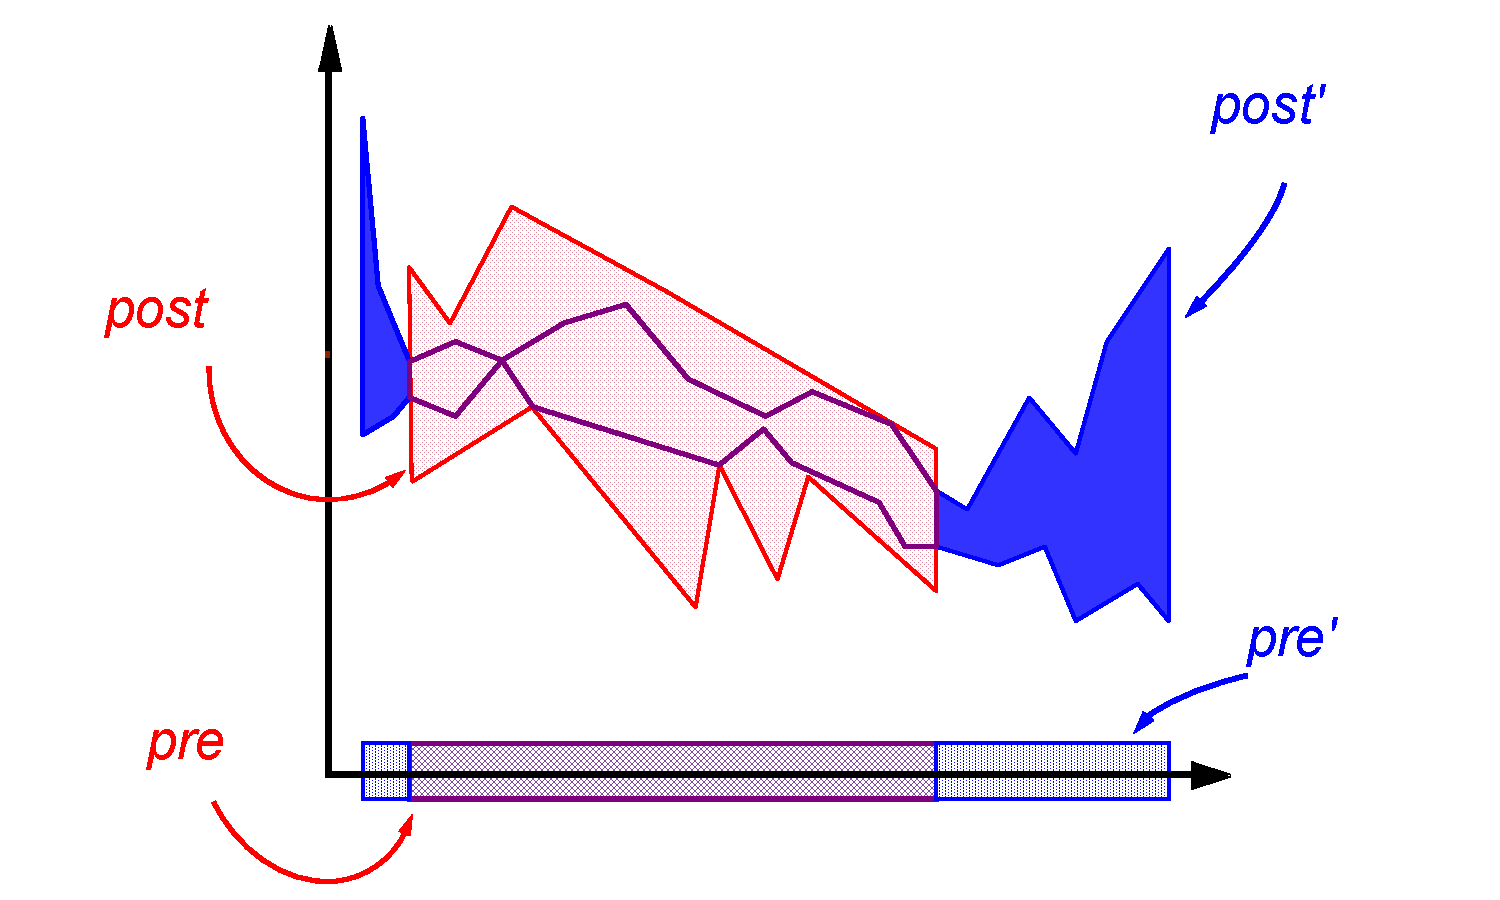
\includegraphics[width=4.25in]{meth-refine3}
\end{frame}

\begin{frame}
\frametitle{Proving Method Refinements}
\begin{theorem}
\label{th:refinement}
Suppose \BLUE{$T' \At (\pre',\post')$} and \RED{$T \At (\pre,\post)$}
specify $m$.

Then 

\begin{displaymath}
\BLUE{(\pre',\post')} \refines^{\BLUETP} \RED{(\pre,\post)}
\end{displaymath}

if and only if:

\begin{displaymath}
\Spec{{\BLUETP}} \Proves
 \RED{\pre} \mbox{ \texttt{\&\&} }
          \mbox{\texttt{(}\textbf{\texttt{this instanceof}} \BLUETP\texttt{)}}
 \Rightarrow \BLUE{\pre'}
\end{displaymath}

and

\begin{displaymath}
\Spec{{\BLUETP}} \Proves
\begin{array}[t]{l}
\mbox{\texttt{{\textbackslash}\textbf{old}(}}\RED{\pre}
   \mbox{ \texttt{\&\&} }
   \mbox{\texttt{(}\textbf{\texttt{this instanceof}} \BLUETP\texttt{))}} \\
   \Rightarrow (\BLUE{\post'} \Rightarrow \RED{\post}).
\end{array}
\end{displaymath}
\end{theorem}
\end{frame}

\begin{frame}
\frametitle{\JMLKW{also} Makes Refinements}

\begin{theorem}
Suppose \mbox{\texttt{{\textbackslash}\textbf{old}}}
is monotonic.
Suppose $\BLUETP \STO \REDT$, and
\BLUE{$T' \At (\pre',\post')$} and \RED{$T \At (\pre,\post)$}
specify $m$.

Then 
\begin{displaymath}
(\BLUE{(\pre',\post')} \join^{\BLUETP} \RED{(\pre,\post)}) 
  \refines^{\BLUETP} \RED{(\pre,\post)}.
\end{displaymath}
\end{theorem}
\note{The proof is direct from the previous theorem.}
\end{frame}

\begin{frame}
\frametitle{Semantics of Multiple Cases}
\transdissolve[duration=0.5]
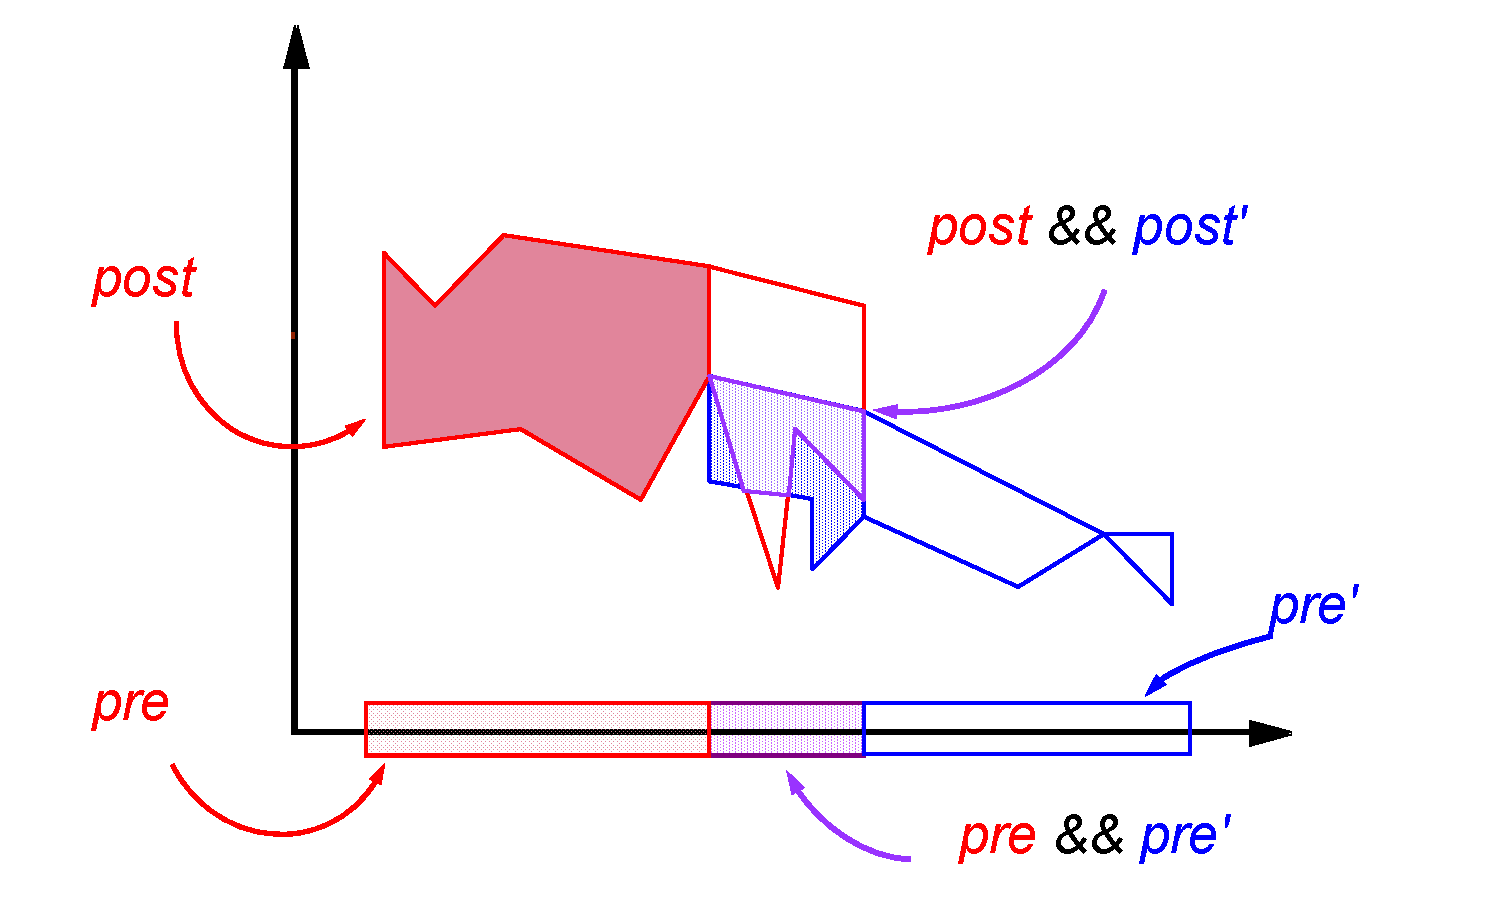
\includegraphics[width=4.25in]{join-both}
\end{frame}

\begin{frame}
\frametitle{Semantics of Multiple Cases}
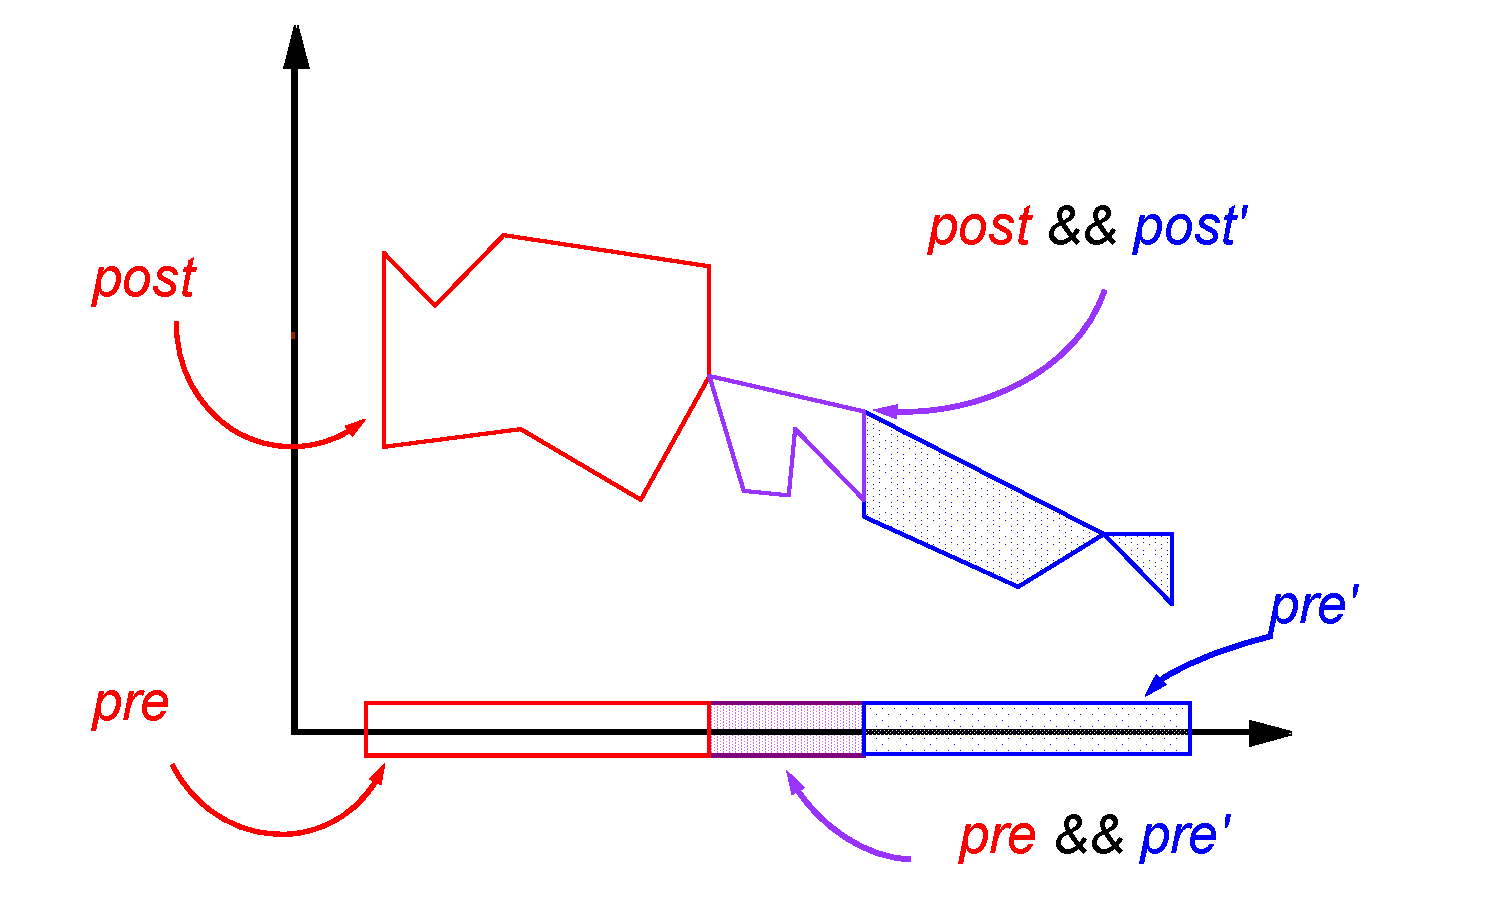
\includegraphics[width=4.25in]{join-intersect}
\end{frame}

\begin{frame}
\frametitle{Spec.~Inheritance Forces Behavioral Subtyping}
\begin{theorem}
Suppose $\BLUETP \STO \REDT$.
Then the extended specification of $\BLUETP$
is a strong behavioral subtype of
the extended specification of $\REDT$.
\end{theorem}
\note{Proof: Use the second theorem above
      and definition of extended specification.
}
\end{frame}

\begin{frame}
\frametitle{Discussion}
\framesubtitle{Behavioral Subtyping and Spec.~Inheritance}

In JML:
\begin{itemize}
\item
Every subtype inherits.

\item
Every subtype is a behavioral subtype.
\begin{itemize}
\item
Not all satisfiable.

\item
Supertype must allow refinement
\end{itemize}
\end{itemize}
\end{frame}

\begin{frame}
\frametitle{Unsatisfiable Refinements}
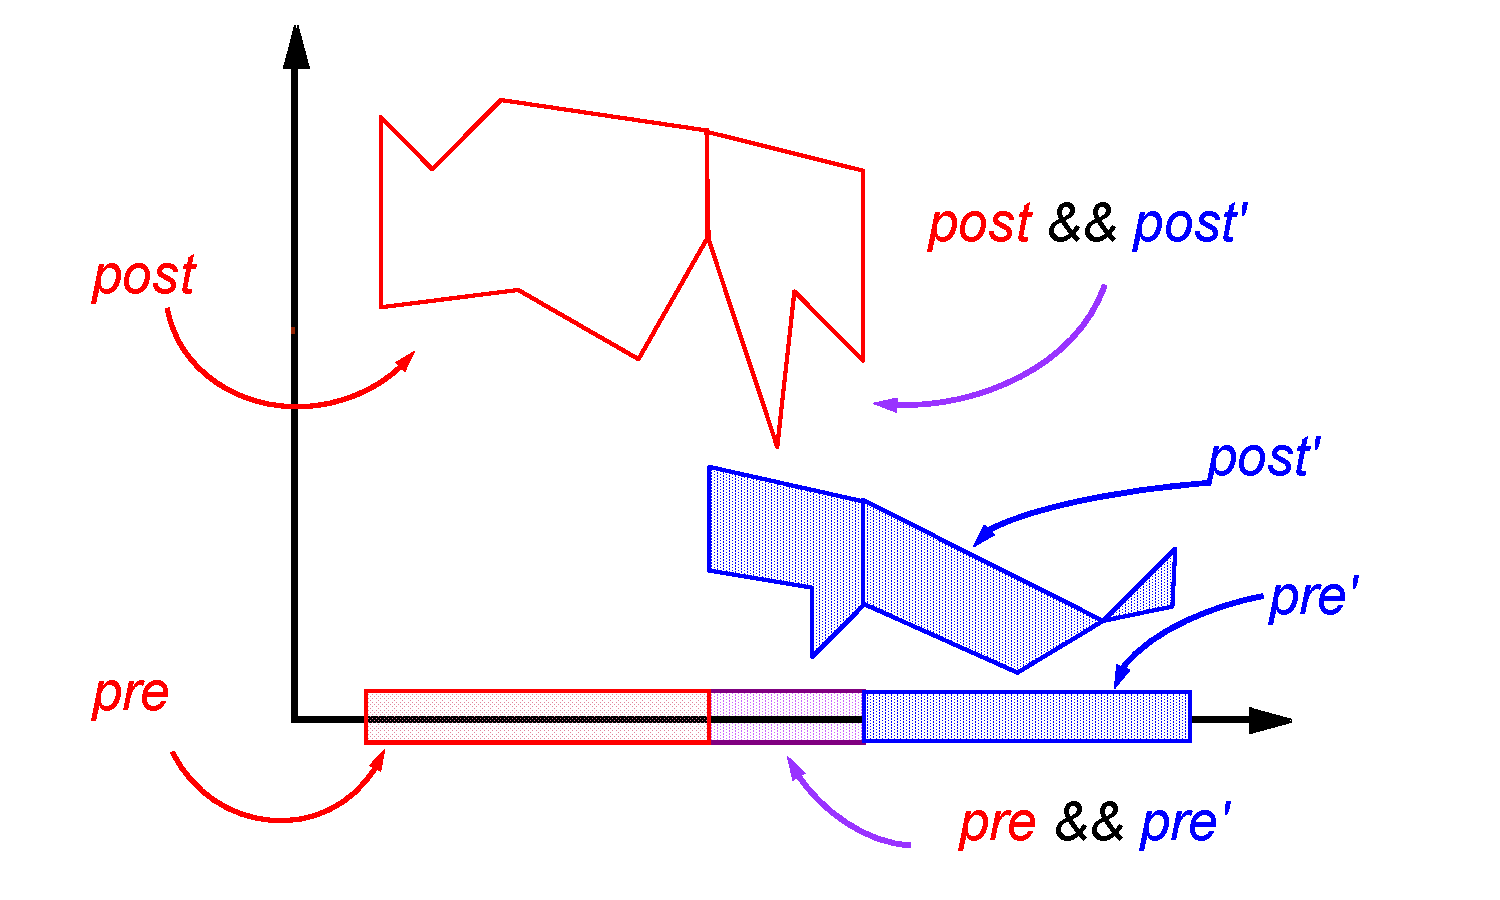
\includegraphics[width=4.25in]{unsatisfiable}
\end{frame}

\begin{frame}
\frametitle{Unsatisfiable Refinements}
\transdissolve[duration=0.5]
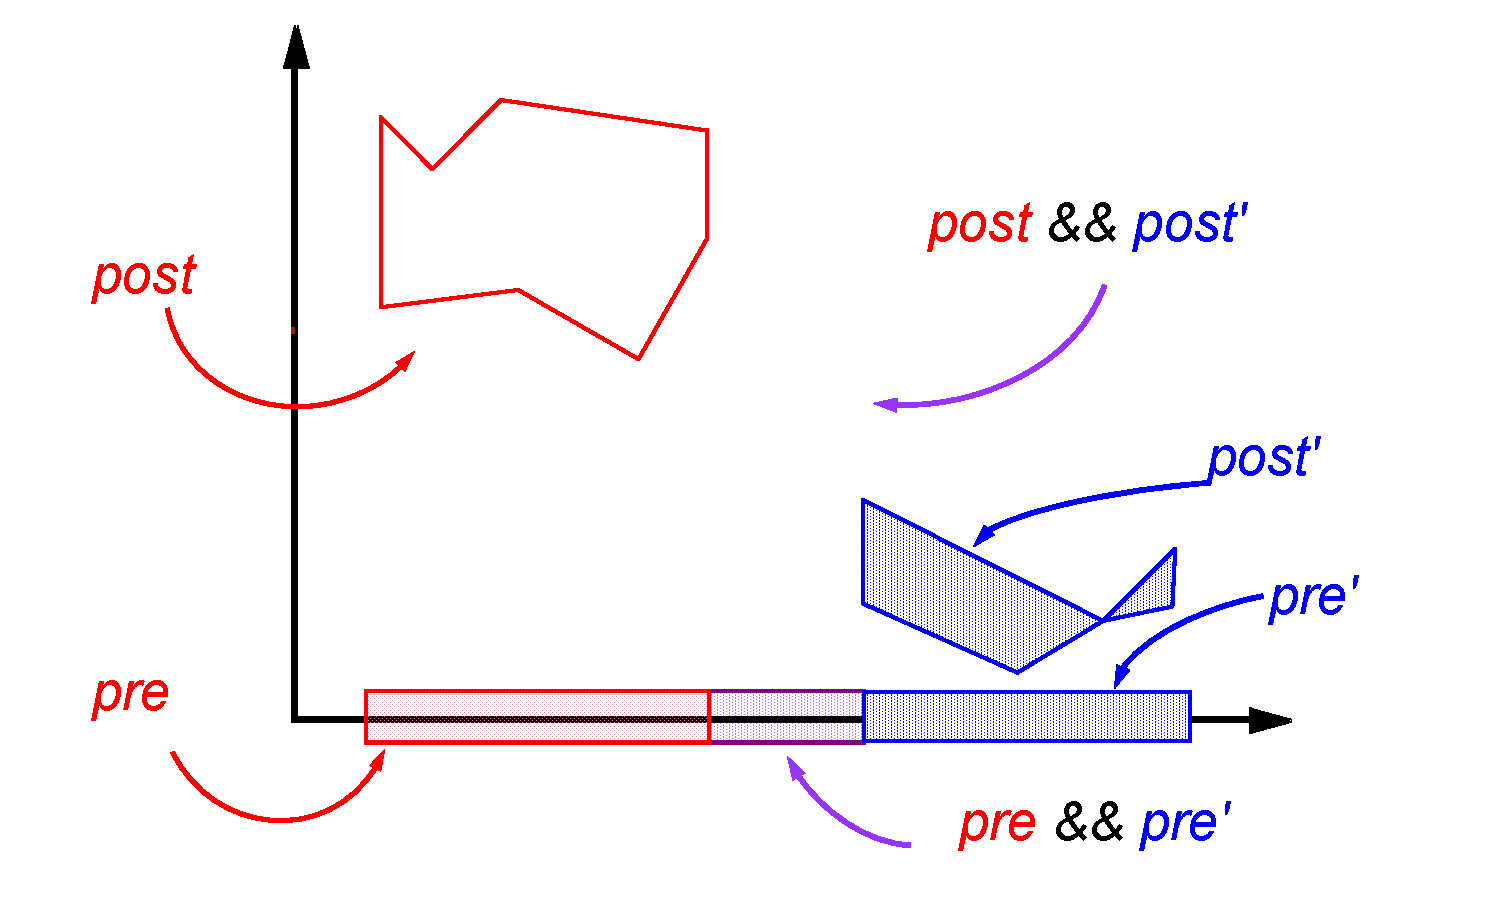
\includegraphics[width=4.25in]{unsatisfiable2}
\end{frame}

\begin{frame}[fragile]
\frametitle{Binary Method Specification}
\begin{question}
What is wrong specifying \lstinline!Gender!'s \lstinline!equals!
method as follows?

\rm
\lstinputlisting[linerange={2-9}]{examples/GenderedEqualsBad.java}
\end{question}
\end{frame}

\begin{frame}<beamer>
\frametitle{What's Wrong With It?}
\begin{itemize}
\item
Says that only gender matters.

\item
Refinements \alert{can't} use other attributes.
\end{itemize}
\end{frame}

\begin{frame}<beamer>
\frametitle{Bad Equals Specification}
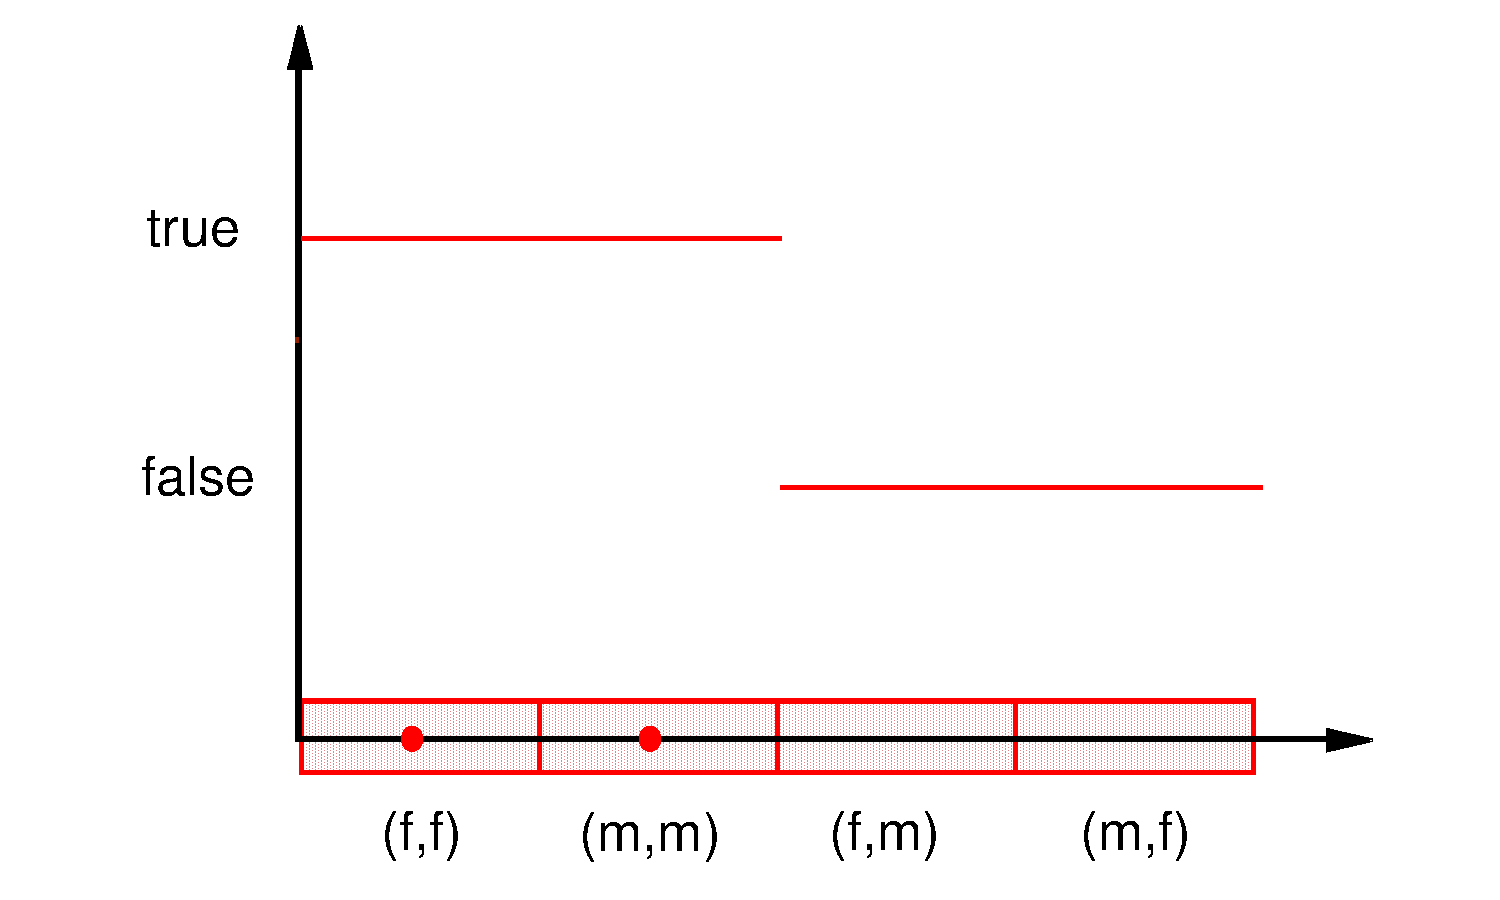
\includegraphics[width=4.25in]{equalsbad1}
\end{frame}

\begin{frame}<beamer>
\frametitle{Bad Equals Specification}
\transdissolve[duration=0.5]
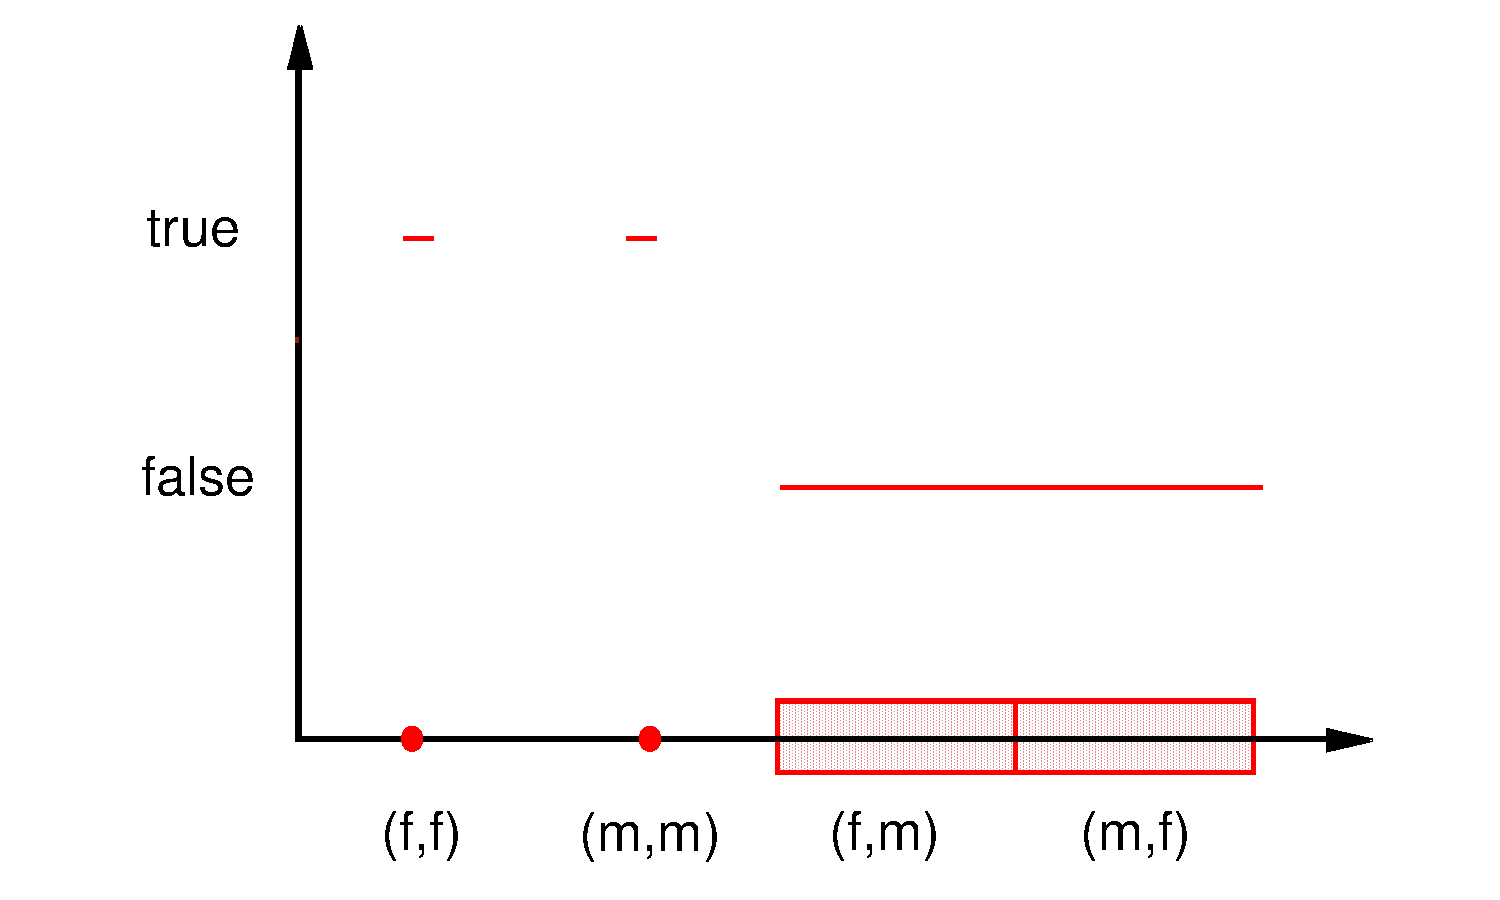
\includegraphics[width=4.25in]{equalsbad2}
\end{frame}

\begin{frame}
\frametitle{Binary Method Specification}
\begin{question}
How to fix it?

\rm
\lstinputlisting[linerange={2-9}]{examples/GenderedEqualsBad.java}
\end{question}
\end{frame}

\begin{frame}<beamer>
\frametitle{Better, Refinable Specification}
\framesubtitle{Using Underspecification}
\lstinputlisting[linerange={2-9}]{examples/GenderedEqualsGood.java}
\note{This says that the gender must be equal.
But allows refinements to use other attributes.
}
\end{frame}

\begin{frame}<beamer>
\frametitle{Better, Refinable Specification}
\framesubtitle{Using Underspecification}
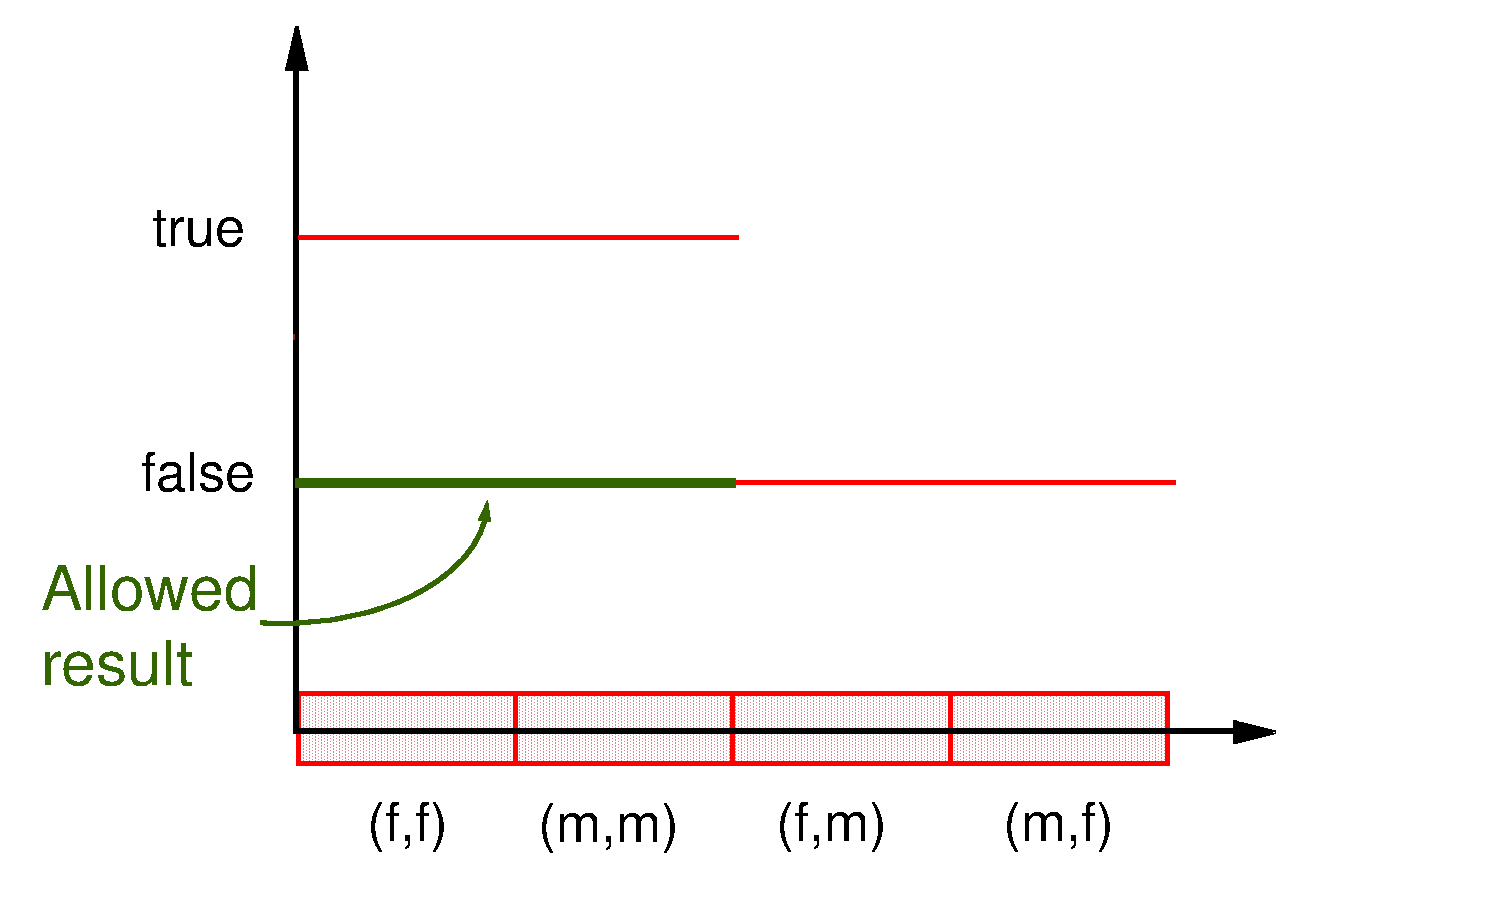
\includegraphics[width=4.25in]{equalsgood}
\end{frame}

\begin{frame}
\frametitle{Conclusions About Subtyping}
\begin{itemize}
\item
Supertype abstraction allows modular reasoning.

\item
Supertype abstraction is valid if:
\begin{itemize}
\item
methodology enforced, and

\item
subtypes are behavioral subtypes.
\end{itemize}

\item
JML's \JMLKW{also} makes refinements.

\item
Specification inheritance in JML
forces behavioral subtyping.

\item
Supertype abstraction 
automatically valid in JML.

\item
Supertype specifications must be permissive.
\end{itemize}
\end{frame}

\section[Concl.]{Conclusions}

\againframe<2>{advantages}

\againframe<2>{opportunities}

\begin{frame}
\frametitle{Current Research on JML}

Semantics and Design Work:
\begin{itemize}
\item
Ownership and invariants (Peter M\"{u}ller, Spec\# folks)

\item
Multithreading (KSU group, INRIA).

\item
Frameworks, callbacks (Steve Shaner, David Naumann, me)
\end{itemize}

Tool Work
\begin{itemize}
\item
Mobius effort (Joe Kiniry and others)

\item
Annotation Support (Jass group, Kristina Boysen)

\item
Testing (Mark Utting, Yoonsik Cheon, $\ldots$).
\end{itemize}
\end{frame}


\begin{frame}
\frametitle{Future Work on JML}
\begin{itemize}
\item
Tools.

\item
Java 1.5 support.

\item
Eclipse support.

\item
Documentation.

\item
Concurrency support.

\item
Semantic details.

\item
Theorem proving tie-ins, Static analysis tie-ins.

\item
Inference of specifications.

\item
Tools that give more benefits.
\end{itemize}
\end{frame}

\begin{frame}
\frametitle{What Are You Interested In?}

\begin{question}
What kinds of research or collaborations interest you?
\end{question}
\end{frame}


\begin{frame}
\frametitle{Acknowledgments}
Thanks to Joseph Kiniry, Erik Poll, David Cok, David Naumann, 
Yoonsik Cheon, Curtis Clifton, Clyde Ruby, Patrice Chalin,
Peter M\"{u}ller, Werner Dietl,
Arnd Poetzsch-Heffter,
Rustan Leino, 
Al Baker, Don Pigozzi,
and
the rest of the JML community.

Join us at$\ldots$

\begin{center}
\href{http://www.jmlspecs.org/}{jmlspecs.org}
\end{center}
\end{frame}


\appendix



\begin{frame}
\frametitle{Modular Reasoning}
\begin{itemize}
\item
Prove code using specifications of other modules.

\item
Sound, if each module satisfies specification.
\end{itemize}

~ 

Scales better than whole-program reasoning.
\end{frame}

\begin{frame}[fragile]
\frametitle{Supertype Abstraction for Initially}
Given:
\lstinputlisting[linerange={2-2,5-6}]{examples/Patient.java}

Verify:
\begin{lstlisting}
  Patient p;
  if (b) { p = new Patient("male"); }
  else { p = new FemalePatient(); }
  //@ assert p.log.size() == 0;
\end{lstlisting}
\note{This works because the initially clause of Patient also applies
  to FemalePatient.
}
\end{frame}

\end{document}
